% Options for packages loaded elsewhere
\PassOptionsToPackage{unicode}{hyperref}
\PassOptionsToPackage{hyphens}{url}
%
\documentclass[
]{article}
\usepackage{amsmath,amssymb}
\usepackage{lmodern}
\usepackage{ifxetex,ifluatex}
\ifnum 0\ifxetex 1\fi\ifluatex 1\fi=0 % if pdftex
  \usepackage[T1]{fontenc}
  \usepackage[utf8]{inputenc}
  \usepackage{textcomp} % provide euro and other symbols
\else % if luatex or xetex
  \usepackage{unicode-math}
  \defaultfontfeatures{Scale=MatchLowercase}
  \defaultfontfeatures[\rmfamily]{Ligatures=TeX,Scale=1}
\fi
% Use upquote if available, for straight quotes in verbatim environments
\IfFileExists{upquote.sty}{\usepackage{upquote}}{}
\IfFileExists{microtype.sty}{% use microtype if available
  \usepackage[]{microtype}
  \UseMicrotypeSet[protrusion]{basicmath} % disable protrusion for tt fonts
}{}
\makeatletter
\@ifundefined{KOMAClassName}{% if non-KOMA class
  \IfFileExists{parskip.sty}{%
    \usepackage{parskip}
  }{% else
    \setlength{\parindent}{0pt}
    \setlength{\parskip}{6pt plus 2pt minus 1pt}}
}{% if KOMA class
  \KOMAoptions{parskip=half}}
\makeatother
\usepackage{xcolor}
\IfFileExists{xurl.sty}{\usepackage{xurl}}{} % add URL line breaks if available
\IfFileExists{bookmark.sty}{\usepackage{bookmark}}{\usepackage{hyperref}}
\hypersetup{
  pdftitle={Problem Set 4},
  pdfauthor={Answer Key},
  hidelinks,
  pdfcreator={LaTeX via pandoc}}
\urlstyle{same} % disable monospaced font for URLs
\usepackage[margin=1in]{geometry}
\usepackage{color}
\usepackage{fancyvrb}
\newcommand{\VerbBar}{|}
\newcommand{\VERB}{\Verb[commandchars=\\\{\}]}
\DefineVerbatimEnvironment{Highlighting}{Verbatim}{commandchars=\\\{\}}
% Add ',fontsize=\small' for more characters per line
\usepackage{framed}
\definecolor{shadecolor}{RGB}{248,248,248}
\newenvironment{Shaded}{\begin{snugshade}}{\end{snugshade}}
\newcommand{\AlertTok}[1]{\textcolor[rgb]{0.94,0.16,0.16}{#1}}
\newcommand{\AnnotationTok}[1]{\textcolor[rgb]{0.56,0.35,0.01}{\textbf{\textit{#1}}}}
\newcommand{\AttributeTok}[1]{\textcolor[rgb]{0.77,0.63,0.00}{#1}}
\newcommand{\BaseNTok}[1]{\textcolor[rgb]{0.00,0.00,0.81}{#1}}
\newcommand{\BuiltInTok}[1]{#1}
\newcommand{\CharTok}[1]{\textcolor[rgb]{0.31,0.60,0.02}{#1}}
\newcommand{\CommentTok}[1]{\textcolor[rgb]{0.56,0.35,0.01}{\textit{#1}}}
\newcommand{\CommentVarTok}[1]{\textcolor[rgb]{0.56,0.35,0.01}{\textbf{\textit{#1}}}}
\newcommand{\ConstantTok}[1]{\textcolor[rgb]{0.00,0.00,0.00}{#1}}
\newcommand{\ControlFlowTok}[1]{\textcolor[rgb]{0.13,0.29,0.53}{\textbf{#1}}}
\newcommand{\DataTypeTok}[1]{\textcolor[rgb]{0.13,0.29,0.53}{#1}}
\newcommand{\DecValTok}[1]{\textcolor[rgb]{0.00,0.00,0.81}{#1}}
\newcommand{\DocumentationTok}[1]{\textcolor[rgb]{0.56,0.35,0.01}{\textbf{\textit{#1}}}}
\newcommand{\ErrorTok}[1]{\textcolor[rgb]{0.64,0.00,0.00}{\textbf{#1}}}
\newcommand{\ExtensionTok}[1]{#1}
\newcommand{\FloatTok}[1]{\textcolor[rgb]{0.00,0.00,0.81}{#1}}
\newcommand{\FunctionTok}[1]{\textcolor[rgb]{0.00,0.00,0.00}{#1}}
\newcommand{\ImportTok}[1]{#1}
\newcommand{\InformationTok}[1]{\textcolor[rgb]{0.56,0.35,0.01}{\textbf{\textit{#1}}}}
\newcommand{\KeywordTok}[1]{\textcolor[rgb]{0.13,0.29,0.53}{\textbf{#1}}}
\newcommand{\NormalTok}[1]{#1}
\newcommand{\OperatorTok}[1]{\textcolor[rgb]{0.81,0.36,0.00}{\textbf{#1}}}
\newcommand{\OtherTok}[1]{\textcolor[rgb]{0.56,0.35,0.01}{#1}}
\newcommand{\PreprocessorTok}[1]{\textcolor[rgb]{0.56,0.35,0.01}{\textit{#1}}}
\newcommand{\RegionMarkerTok}[1]{#1}
\newcommand{\SpecialCharTok}[1]{\textcolor[rgb]{0.00,0.00,0.00}{#1}}
\newcommand{\SpecialStringTok}[1]{\textcolor[rgb]{0.31,0.60,0.02}{#1}}
\newcommand{\StringTok}[1]{\textcolor[rgb]{0.31,0.60,0.02}{#1}}
\newcommand{\VariableTok}[1]{\textcolor[rgb]{0.00,0.00,0.00}{#1}}
\newcommand{\VerbatimStringTok}[1]{\textcolor[rgb]{0.31,0.60,0.02}{#1}}
\newcommand{\WarningTok}[1]{\textcolor[rgb]{0.56,0.35,0.01}{\textbf{\textit{#1}}}}
\usepackage{longtable,booktabs,array}
\usepackage{calc} % for calculating minipage widths
% Correct order of tables after \paragraph or \subparagraph
\usepackage{etoolbox}
\makeatletter
\patchcmd\longtable{\par}{\if@noskipsec\mbox{}\fi\par}{}{}
\makeatother
% Allow footnotes in longtable head/foot
\IfFileExists{footnotehyper.sty}{\usepackage{footnotehyper}}{\usepackage{footnote}}
\makesavenoteenv{longtable}
\usepackage{graphicx}
\makeatletter
\def\maxwidth{\ifdim\Gin@nat@width>\linewidth\linewidth\else\Gin@nat@width\fi}
\def\maxheight{\ifdim\Gin@nat@height>\textheight\textheight\else\Gin@nat@height\fi}
\makeatother
% Scale images if necessary, so that they will not overflow the page
% margins by default, and it is still possible to overwrite the defaults
% using explicit options in \includegraphics[width, height, ...]{}
\setkeys{Gin}{width=\maxwidth,height=\maxheight,keepaspectratio}
% Set default figure placement to htbp
\makeatletter
\def\fps@figure{htbp}
\makeatother
\setlength{\emergencystretch}{3em} % prevent overfull lines
\providecommand{\tightlist}{%
  \setlength{\itemsep}{0pt}\setlength{\parskip}{0pt}}
\setcounter{secnumdepth}{-\maxdimen} % remove section numbering
\usepackage{amsmath}
\usepackage{multirow, multicol, booktabs}
\usepackage{array}
\usepackage{caption}
\usepackage{graphicx}
\usepackage{siunitx}
\usepackage[normalem]{ulem}
\usepackage{colortbl}
\usepackage{multirow}
\usepackage{hhline}
\usepackage{calc}
\usepackage{tabularx}
\usepackage{threeparttable}
\usepackage{wrapfig}
\usepackage{adjustbox}
\usepackage{hyperref}
\ifluatex
  \usepackage{selnolig}  % disable illegal ligatures
\fi

\title{Problem Set 4}
\author{Answer Key}
\date{ECON 480 --- Fall 2021}

\begin{document}
\maketitle

Answers generally go above and beyond what I expect from you. They are
meant to show you the correct answer, explain \emph{why} it is correct,
and potentially show \emph{several methods} by which you can reach the
answer.

\hypertarget{theory-and-concepts}{%
\section{Theory and Concepts}\label{theory-and-concepts}}

\hypertarget{question-1}{%
\subsection{Question 1}\label{question-1}}

\textbf{In your own words, explain the fundamental problem of causal
inference.}

\begin{center}\rule{0.5\linewidth}{0.5pt}\end{center}

The fundamental problem of causal inference is that we never know the
counterfactuals for the observations that we actually see in the data. A
causal effect of a treatment \((\delta_i)\) for individual \(i\) would
be the difference between their outcomes if they were treated
\((Y^1_i)\) and if they were not-treated \((Y^0_i)\),
i.e.~\(\delta_i=Y^1_i-Y^0_i\). Across many individuals, we could take
the average for each group (treated and untreated group). However, in
reality, for each individual in our data, we only ever see \(Y^1_i\)
\emph{or} \(Y^0_i\), \emph{never both}. We only see a person's outcome
with treatment, or without treatment, so we cannot simply take the
difference.

\begin{center}\rule{0.5\linewidth}{0.5pt}\end{center}

\hypertarget{question-2}{%
\subsection{Question 2}\label{question-2}}

\textbf{In your own words, explain how properly conducting a randomized
controlled trial helps to identify the causal effect of one variable on
another.}

\begin{center}\rule{0.5\linewidth}{0.5pt}\end{center}

Randomized controlled experiments are where a pool of subjects
representative of a population are randomly assigned into a treatment
group (or into one of a number of groups given different levels of a
treatment) or into a control group. The treatment group(s) is(are) given
the treatment(s), the control group is given nothing (perhaps a placebo,
though this is not always necessary), and then the average results of
the two groups are compared to measure the true average effect of
treatment.

The key is that the assignment must be random, which controls for all
factors that potentially determine the outcome (e.g.~when measuring
individual outcomes, their height, family background, income, race, age,
etc). If subjects are randomly assigned, then knowing anything about the
individual (e.g.~age, height, etc) tells us nothing about whether or not
they got the treatment(s). The only thing that separates a member of the
treatment group(s) from the control group is whether or not they were
assigned to treatment. This ensures that the average person in the
treatment group(s) looks like the average person in the control group,
and that we are truly comparing apples to apples, rather than apples to
oranges.

\begin{center}\rule{0.5\linewidth}{0.5pt}\end{center}

\hypertarget{question-3}{%
\subsection{Question 3}\label{question-3}}

\textbf{In your own words, describe what omitted variable bias means.
What are the two conditions for a variable to bias OLS estimates if
omitted?}

\begin{center}\rule{0.5\linewidth}{0.5pt}\end{center}

All variables that might influence the dependent variable (\(Y\)) that
we do not measure and include in our regression are a part of the error
term \((\epsilon\)). If we omit a variable \((Z)\), it will cause a bias
if and only if it meets both of the following conditions: 1. The
variable must be a determinant of our dependent variable,
\(corr(Z,Y)\neq 0\), and thus would appear in the error term,
\(\epsilon\). 2. The variable must be correlated with one of our
independent variables of interest in our regression,
\(corr(Z,X) \neq 0\).

If both conditions are met, then if we did not include the omitted
variable \(Z\), our estimate of the causal effect of \(X\) on \(Y\)
would be biased, because our estimate \((\hat{\beta_1}\)) would pick up
some of the effect of \(Z\). If we include \(Z\) as another independent
variable, then the \(\hat{\beta_1}\) on \(X\) will tell us the precise
effect of \emph{only} \(X\rightarrow Y\), holding \(Z\) constant.

\begin{verbatim}
## -- Attaching packages --------------------------------------- tidyverse 1.3.1 --
\end{verbatim}

\begin{verbatim}
## v ggplot2 3.3.5     v purrr   0.3.4
## v tibble  3.1.5     v dplyr   1.0.7
## v tidyr   1.1.3     v stringr 1.4.0
## v readr   2.0.0     v forcats 0.5.1
\end{verbatim}

\begin{verbatim}
## -- Conflicts ------------------------------------------ tidyverse_conflicts() --
## x dplyr::filter() masks stats::filter()
## x dplyr::lag()    masks stats::lag()
\end{verbatim}

\begin{verbatim}
## 
## Attaching package: 'ggdag'
\end{verbatim}

\begin{verbatim}
## The following object is masked from 'package:stats':
## 
##     filter
\end{verbatim}

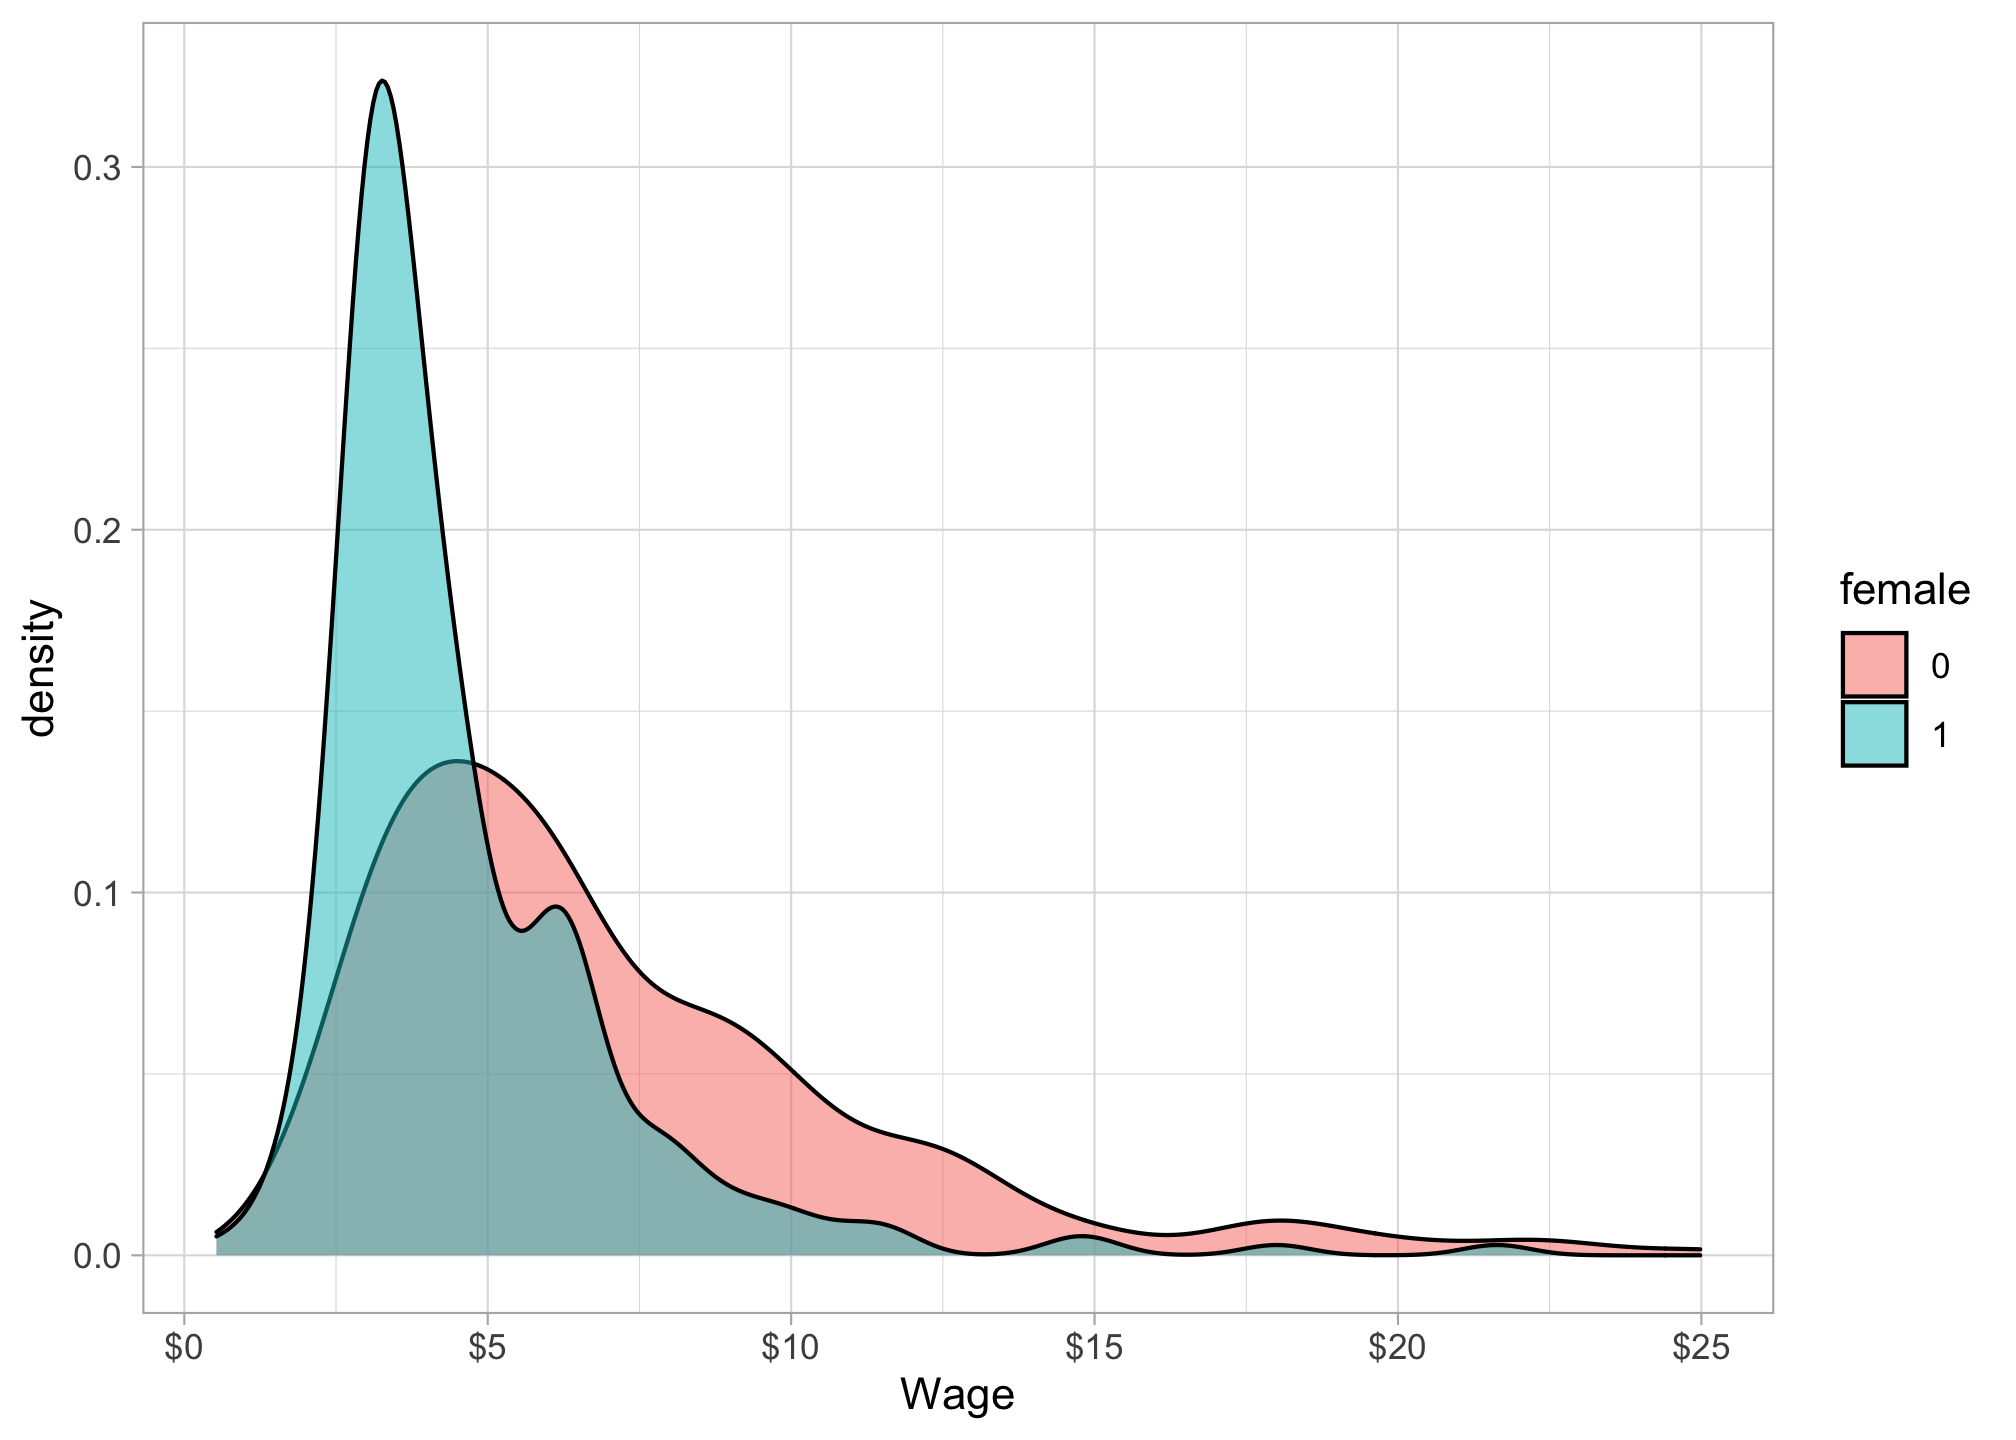
\includegraphics[width=0.8\linewidth]{04-problem-set-answers-pdf_files/figure-latex/unnamed-chunk-2-1}

\begin{center}\rule{0.5\linewidth}{0.5pt}\end{center}

\hypertarget{question-4}{%
\subsection{Question 4}\label{question-4}}

\textbf{In your own words, describe what multicollinearity means. What
is the cause, and what are the consequences of multicollinearity? How
can we measure multicollinearity and its effects? What happens if
multicollinearity is \emph{perfect}?}

\begin{center}\rule{0.5\linewidth}{0.5pt}\end{center}

Multicollinearity just means that two regressors (e.g .\(X_1\) and
\(X_2\)) are correlated with each other. This fact does \emph{not} bias
the OLS estimates of these regressors (e.g.~\(\hat{\beta_1}\) and
\(\hat{\beta_2}\)). In fact, the reason \(X_2\) is included in the
regression is because omitting it would cause omitted variable bias,
since \(corr(X_1,X_2)\neq 0\) and \(corr(Y, X_2)\neq 0\). However, the
variance of these OLS estimators is increased because it is hard to get
a precise measure of \(X_1\rightarrow Y\) because \(X_2\rightarrow Y\)
also, and \(X_1\) may tend to be certain values (large or small) when
\(X_2\) is certain values (large or small) so we don't know
counterfactuals (e.g.~what if \(X_1\) were the \emph{opposite} of what
it tends to be (large or small) when \(X_2\) is large or small).

The strength of multicollinearity is simply given by the value of the
correlation coefficient between \(X_1\) and \(X_2\), \(r_{X_1,X_2}\). We
can measure the \emph{effect} of multicollinearity on the variance of a
regressor (\(X_j\))'s coefficient (\(\hat{\beta_j}\)) with the
\textbf{Variance Inflation Factor}:

\[VIF=\frac{1}{1-R^2_j}\]

where \(R^2_j\) is the \(R^2\) from an auxiliary regression of \(X_j\)
on all of the other regressors.

Multicollinearity is \emph{perfect} when the correlation between \(X_1\)
and \(X_2\) is 1 or -1. This happens when one regressor (e.g.~\(X_1\))
is an exact linear function of another regressor(s)
\((e.g. X_1=\frac{X_2}{100}\). A regression cannot be run including both
variables, as it creates a logical contradiction. In this example,
\(\hat{\beta_1}\) would be the marginal effect on \(Y\) of changing
\(X_1\) holding \(X_2\) constant -- but \(X_2\) would naturally change
as it is a function of \(X_1\)!

\begin{center}\rule{0.5\linewidth}{0.5pt}\end{center}

\hypertarget{question-5}{%
\subsection{Question 5}\label{question-5}}

\textbf{Explain how we use Directed Acyclic Graphs (DAGs) to depict a
causal model: what are the two criteria that must hold for identifying a
causal effect of \(X\) on \(Y\)? When should we control a variable, and
when should we \emph{not} control for a variable?}

\begin{center}\rule{0.5\linewidth}{0.5pt}\end{center}

A Directed Acyclic Graph (DAG) describes a causal model based on making
our assumptions about relationships between variables explicit, and in
many cases, testable.

Variables are represented as nodes, and causal effects represented as
arrows from one node to another (in the direction of the causal effect).
We think about the causal effect of \(X \rightarrow Y\) in
\emph{counterfactual} terms: if \(X\) had been different, \(Y\) would
have been different as a response.

When considering the causal effect of \(X \rightarrow Y\), we must
consider \emph{all pathways from \(X\) to \(Y\)} (that do not loop, or
go through a variable twice), regardless of the direction of the arrows.
The paths will be of two types:

\begin{itemize}
\tightlist
\item
  \textbf{Causal (front-door) pathways} where arrows go from \(X\) into
  \(Y\) (including through other \textbf{mediator} variables)
\item
  \textbf{Non-causal (back-door) pathways} where an arrow leads into
  \(X\) (implying \(X\) is partially caused by that variable)
\end{itemize}

Adjusting or controlling for (in a multivariate regression, this means
including the variable in the regression) a variable along a pathway
closes that pathway.

Variables should be adjusted (controlled for) such that:

\begin{enumerate}
\def\labelenumi{\arabic{enumi}.}
\tightlist
\item
  \textbf{Back-door criterion}: no backdoor pathway between \(X\) and
  \(Y\) remains open
\item
  \textbf{Front-door criterion}: no frontdoor pathway is closed
\end{enumerate}

The one exception is a \textbf{collider} variable, where a variable
along a pathway has arrows pointing into it from both directions. This
\emph{automatically blocks a path} (whether front door or back door).
Controlling for a collider variable \emph{opens} the pathway it is on.

See \href{/r/3.2-r-answers.Rmd}{R Practice on Causality and DAGs} for
examples.

\begin{center}\rule{0.5\linewidth}{0.5pt}\end{center}

\hypertarget{theory-problems}{%
\section{Theory Problems}\label{theory-problems}}

For the following questions, please \emph{show all work} and explain
answers as necessary. You may lose points if you only write the correct
answer. You may use \texttt{R} to \emph{verify} your answers, but you
are expected to reach the answers in this section ``manually.''

\hypertarget{question-6}{%
\subsection{Question 6}\label{question-6}}

A pharmaceutical company is interested in estimating the impact of a new
drug on cholesterol levels. They enroll 200 people in a clinical trial.
People are randomly assigned the treatment group or into the control
group. Half of the people are given the new drug and half the people are
given a sugar pill with no active ingredient. To examine the impact of
dosage on reductions in cholesterol levels, the authors of the study
regress the following model:

\[\text{cholesterol level}_i = \beta_0+\beta_1 \text{dosage level}_i + u_i\]

For people in the control group, dosage level\(_i=0\) and for people in
the treatment group, dosage level\(_i\) measures milligrams of the
active ingredient. In this case, the authors find a large, negative,
statistically significant estimate of \(\hat{\beta_1}\). Is this an
unbiased estimate of the impact of dosage on change in cholesterol
level? Why or why not? Do you expect the estimate to overstate or
understate the true relationship between dosage and cholesterol level?

\begin{center}\rule{0.5\linewidth}{0.5pt}\end{center}

Consider the 4th assumption about the error term, \(u_i\). Does knowing
whether (or how much) a person was treated convey any information about
other characteristics that affect cholesterol level (in \(u_i\))? Again,
we are asking if \(E[u|X]=0\) or \(cor(X, u)=0\).

In this case, the answer is clearly no; knowing whether or not someone
received treatment tells us \emph{nothing} else about the person that
might affect their cholesterol levels (i.e.~age, height, diet, weight,
family history, etc., all in \(u_i)\) because treatment is
\emph{randomly} assigned.

In this case, because treatment is exogenous,
\(E[\hat{\beta_1}]=\beta_1\), \(\hat{\beta_1}\) is unbiased.

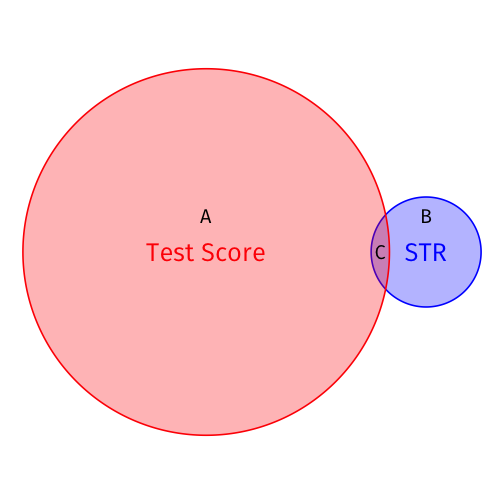
\includegraphics[width=0.8\linewidth]{04-problem-set-answers-pdf_files/figure-latex/unnamed-chunk-3-1}

\begin{center}\rule{0.5\linewidth}{0.5pt}\end{center}

\hypertarget{question-7}{%
\subsection{Question 7}\label{question-7}}

Data were collected from a random sample of 220 home sales from a
community in 2017.

\[\widehat{Price}=119.2+0.485 \, BDR+23.4 \, Bath+0.156 \, Hsize+0.002 \, Lsize+0.090 \, Age\]

\begin{longtable}[]{@{}ll@{}}
\toprule
Variable & Description \\
\midrule
\endhead
\(Price\) & selling price (in \$1,000s) \\
\(BDR\) & number of bedrooms \\
\(Bath\) & number of bathrooms \\
\(Hsize\) & size of the house (in ft\(^2)\) \\
\(Lsize\) & lot size (in ft\(^2)\) \\
\(Age\) & age of the house (in years) \\
\bottomrule
\end{longtable}

\hypertarget{part-a}{%
\subsubsection{Part A}\label{part-a}}

\textbf{Suppose that a homeowner converts part of an existing living
space in her house to a new bathroom. What is the expected increase in
the value of the house?}

\begin{center}\rule{0.5\linewidth}{0.5pt}\end{center}

From \(\hat{\beta_2}\), \$23,400.

\begin{center}\rule{0.5\linewidth}{0.5pt}\end{center}

\hypertarget{part-b}{%
\subsubsection{Part B}\label{part-b}}

\textbf{Suppose a homeowner adds a new bathroom to her house, which also
increases the size of the house by 100 square feet. What is the expected
increase in the value of the house?}

\begin{center}\rule{0.5\linewidth}{0.5pt}\end{center}

In this case, \(\Delta BDR=1\) and \(\Delta Hsize=100\). The resulting
expected increase in price is \(23.4(1)+0.156(100)=39.0\), or \$39,000.

\begin{center}\rule{0.5\linewidth}{0.5pt}\end{center}

\hypertarget{part-c}{%
\subsubsection{Part C}\label{part-c}}

\textbf{Suppose the \(R^2\) of this regression is 0.727. Calculate the
adjusted \(\bar{R}^2\).}

\begin{center}\rule{0.5\linewidth}{0.5pt}\end{center}

There are \(n=220\) observations and \(k=6\) variables, so:

\[\begin{align*}
\bar{R}^2&=1-\frac{n-1}{n-k-1}(1-R^2)\\
&=1-\frac{220-1}{220-6-1}(1-0.727)\\
&=1-\frac{219}{213}(0.273)\\
&=0.719\\
\end{align*}\]

\begin{center}\rule{0.5\linewidth}{0.5pt}\end{center}

\hypertarget{part-d}{%
\subsubsection{Part D}\label{part-d}}

\textbf{Suppose the following auxiliary regression for \(BDR\) has an
\(R^2\) of 0.841.}

\[\widehat{BDR}=\delta_0+\delta_1Bath+\delta_2Hsize+\delta_3Lsize+\delta_4Age\]

\textbf{Calculate the Variance Inflation Factor for \(BDR\) and explain
what it means.}

\begin{center}\rule{0.5\linewidth}{0.5pt}\end{center}

\[\begin{align*}
VIF&=\frac{1}{1-R^2_j}\\
&=\frac{1}{1-0.841}\\
&=\frac{1}{0.159}\\
&=6.29\\
\end{align*}\]

The variance on \(\hat{\beta_2}\) (on Bath) increases by 6.29 times due
to multicollinearity between Bath and other \(X\)-variables.

\begin{center}\rule{0.5\linewidth}{0.5pt}\end{center}

\hypertarget{question-8}{%
\subsection{Question 8}\label{question-8}}

A researcher wants to investigate the effect of education on average
hourly wages. Wage, education, and experience in the dataset have the
following correlations:

\begin{longtable}[]{@{}lrrr@{}}
\toprule
& Wage & Education & Experience \\
\midrule
\endhead
Wage & 1.0000 & & \\
Education & 0.4059 & 1.0000 & \\
Experience & 0.1129 & -0.2995 & 1.0000 \\
\bottomrule
\end{longtable}

She runs a simple regression first, and gets the results:

\[\widehat{\text{Wage}} = -0.9049 +  0.5414 \, Education\]

She runs another regression, and gets the results:

\[\widehat{\text{Experience}} = 35.4615 - 1.4681 \, Education\]

\hypertarget{part-a-1}{%
\subsubsection{Part A}\label{part-a-1}}

\textbf{If the true marginal effect of experience on wages (holding
education constant) is 0.0701, calculate the omitted variable bias in
the first regression caused by omitting experience. Does the estimate of
\(\hat{\beta_1}\) in the first regression overstate or understate the
effect of education on wages?}

\begin{center}\rule{0.5\linewidth}{0.5pt}\end{center}

We know that the estimate in the biased regression (first one above) is
a function of:

\[\hat{\alpha_1}=\hat{\beta_1}+\hat{\beta_2}\hat{\delta_1}\]

Where:

\begin{itemize}
\tightlist
\item
  \(\hat{\alpha_1}\): the coefficient on education in the biased
  regression (0.5414)
\item
  \(\hat{\beta_1}\): the true effect of education on wages (??)
\item
  \(\hat{\beta_2}\): the true effect of experience on wages (0.0701)
\item
  \(\hat{\delta_1}\): the effect of education on experience (from an
  auxiliary regression) (-1.4681)
\end{itemize}

\[\begin{align*}
        OMV&=\hat{\beta_2} \hat{\delta_1}\\
        &=(0.0701)(-1.4681)\\
        &=-0.1029
\end{align*}\]

Since the bias is negative, it understates the effect of education (due
to experience). Note there are other factors that can bias the effect of
education, but at least through experience, the bias is negative since
the two are negatively related in the data (see the second regression).

\begin{center}\rule{0.5\linewidth}{0.5pt}\end{center}

\hypertarget{part-b-1}{%
\subsubsection{Part B}\label{part-b-1}}

\textbf{Knowing this, what would be the \emph{true effect} of education
on wages, holding experience constant?}

\begin{center}\rule{0.5\linewidth}{0.5pt}\end{center}

We know the biased estimate for education, 0.0611. Plugging in both this
and the bias, we get the ``true'' effect:

\[\begin{align*}
            \alpha_1&=\beta_1+\beta_2\delta_1\\
            0.5414&=\beta_1-0.1029\\
            0.6443&=\beta_1\\
\end{align*}\] ---

\hypertarget{part-c-1}{%
\subsubsection{Part C}\label{part-c-1}}

\textbf{The \(R^2\) for the second regression is 0.0897. If she were to
run a better regression including both education and experience, how
much would the variance of the coefficients on education and experience
increase? Why?}

\begin{center}\rule{0.5\linewidth}{0.5pt}\end{center}

Here we need to calculate the Variance Inflation Factor (VIF) by using
the \(R^2\) from the auxiliary regression.

\[\begin{align*}
        VIF &=\frac{1}{1-R^2_j}\\
        &=\frac{1}{1-(0.0897)}\\
        &=\frac{1}{0.9103}\\
        &=1.0985
\end{align*}\]

The variance increases only by 1.0985 times due to fairly weak
multicollinearity between education and experience.

\begin{center}\rule{0.5\linewidth}{0.5pt}\end{center}

\hypertarget{r-questions}{%
\section{R Questions}\label{r-questions}}

Answer the following questions using \texttt{R}. When necessary, please
write answers in the same document (knitted \texttt{Rmd} to
\texttt{html} or \texttt{pdf}, typed \texttt{.doc(x)}, or handwritten)
as your answers to the above questions. Be sure to include (email or
print an \texttt{.R} file, or show in your knitted \texttt{markdown})
your code and the outputs of your code with the rest of your answers.

\hypertarget{question-9}{%
\subsection{Question 9}\label{question-9}}

Install and load the \texttt{wooldridge} package. This package contains
datasets used in Jeffrey Wooldridge's \emph{Introductory Econometrics: A
Modern Approach} (the textbook that I used in \emph{my} econometrics
classes years ago!).

We will use the \texttt{bwght} data from \texttt{wooldridge}, which
comes from The 1988 National Health Interview Survey., used in J.
Mullahy (1997), ``Instrumental-Variable Estimation of Count Data Models:
Applications to Models of Cigarette Smoking Behavior,'' \emph{Review of
Economics and Statistics} 79: 596-593.

Let's just look at the following variables:

\begin{longtable}[]{@{}ll@{}}
\toprule
Variable & Description \\
\midrule
\endhead
\texttt{bwght} & Birth Weight (ounces) \\
\texttt{cigs} & Cigarettes smoked per day while pregnant (1988) \\
\texttt{motheduc} & Mother's education (number of years) \\
\texttt{cigprice} & Price of cigarette pack (1988) \\
\texttt{faminc} & Family's income in \$1,000s (1988) \\
\bottomrule
\end{longtable}

\begin{quote}
We want to explore how a mother smoking during pregnancy affects the
baby's birthweight (which may have strong effects on outcomes over the
child's life).
\end{quote}

Just to be explicit about it, assign this as some dataframe (feel free
to change the name), i.e.:

\begin{Shaded}
\begin{Highlighting}[]
\CommentTok{\# install.packages("wooldridge")}
\FunctionTok{library}\NormalTok{(wooldridge)}
\NormalTok{births }\OtherTok{\textless{}{-}}\NormalTok{ bwght }\CommentTok{\# feel free to rename whatever you want for the dataframe}
\end{Highlighting}
\end{Shaded}

\hypertarget{part-a-2}{%
\subsubsection{Part A}\label{part-a-2}}

\textbf{Make a correlation table for our variables listed above.}

\textbf{Hint: \texttt{select()} these variables and then pipe this into
\texttt{cor(.,\ use\ =\ "pairwise.complete.obs")} to use only
observations for which there are data on each variable (to avoid
\texttt{NA}'s).}

\begin{center}\rule{0.5\linewidth}{0.5pt}\end{center}

\begin{Shaded}
\begin{Highlighting}[]
\CommentTok{\# install.packages("wooldridge")}
\FunctionTok{library}\NormalTok{(wooldridge)}
\NormalTok{births }\OtherTok{\textless{}{-}}\NormalTok{ bwght }\CommentTok{\# save data}
\end{Highlighting}
\end{Shaded}

\begin{Shaded}
\begin{Highlighting}[]
\NormalTok{bwght }\SpecialCharTok{\%\textgreater{}\%}
  \FunctionTok{select}\NormalTok{(bwght, cigs, motheduc, cigprice, faminc) }\SpecialCharTok{\%\textgreater{}\%}
  \FunctionTok{cor}\NormalTok{(}\AttributeTok{use =} \StringTok{"pairwise.complete.obs"}\NormalTok{)}
\end{Highlighting}
\end{Shaded}

\begin{verbatim}
##                bwght        cigs    motheduc   cigprice      faminc
## bwght     1.00000000 -0.15076180  0.06912704 0.04918790  0.10893684
## cigs     -0.15076180  1.00000000 -0.21386510 0.00970419 -0.17304493
## motheduc  0.06912704 -0.21386510  1.00000000 0.07086587  0.45592970
## cigprice  0.04918790  0.00970419  0.07086587 1.00000000  0.09545581
## faminc    0.10893684 -0.17304493  0.45592970 0.09545581  1.00000000
\end{verbatim}

\begin{center}\rule{0.5\linewidth}{0.5pt}\end{center}

\hypertarget{part-b-2}{%
\subsubsection{Part B}\label{part-b-2}}

\hypertarget{part-b-3}{%
\subsubsection{Part B}\label{part-b-3}}

Consider the following causal model:

\begin{Shaded}
\begin{Highlighting}[]
\FunctionTok{library}\NormalTok{(ggdag)}
\FunctionTok{dagify}\NormalTok{(bwght }\SpecialCharTok{\textasciitilde{}}\NormalTok{ cigs }\SpecialCharTok{+}\NormalTok{ inc,}
\NormalTok{       cigs }\SpecialCharTok{\textasciitilde{}}\NormalTok{ price }\SpecialCharTok{+}\NormalTok{ educ }\SpecialCharTok{+}\NormalTok{ inc,}
\NormalTok{       inc }\SpecialCharTok{\textasciitilde{}}\NormalTok{ educ,}
       \AttributeTok{exposure =} \StringTok{"cigs"}\NormalTok{,}
       \AttributeTok{outcome =} \StringTok{"bwght"}\NormalTok{) }\SpecialCharTok{\%\textgreater{}\%}
  \FunctionTok{tidy\_dagitty}\NormalTok{(}\AttributeTok{seed =} \DecValTok{256}\NormalTok{) }\SpecialCharTok{\%\textgreater{}\%}
  \FunctionTok{ggdag\_status}\NormalTok{()}\SpecialCharTok{+}
  \FunctionTok{theme\_dag\_blank}\NormalTok{()}\SpecialCharTok{+}
  \FunctionTok{theme}\NormalTok{(}\AttributeTok{legend.position =} \StringTok{"none"}\NormalTok{)}
\end{Highlighting}
\end{Shaded}

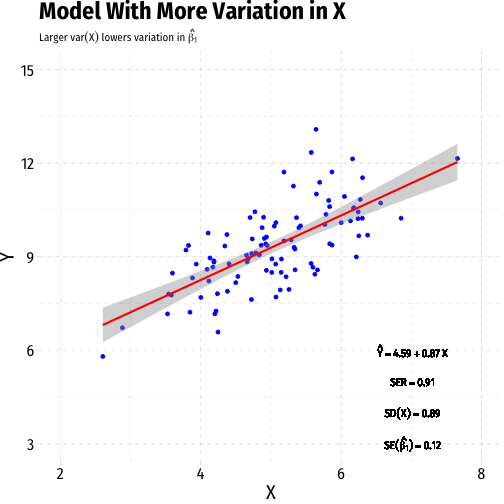
\includegraphics[width=0.8\linewidth]{04-problem-set-answers-pdf_files/figure-latex/unnamed-chunk-7-1}

Note what we are hypothesizing:

\begin{enumerate}
\def\labelenumi{\arabic{enumi}.}
\tightlist
\item
  \texttt{bwght} is caused by \texttt{cigs} and \texttt{inc}
\item
  \texttt{cigs} are caused by \texttt{price}, \texttt{educ}, and
  \texttt{inc}
\item
  \texttt{inc} is caused by \texttt{educ}
\end{enumerate}

See also how this is written into the notation in R to draw (plot) the
DAG.

Create this model on \href{htpp://dagitty.net}{dagitty.net}. What does
\texttt{dagitty} tell us the testable implications of this causal model?

\begin{center}\rule{0.5\linewidth}{0.5pt}\end{center}

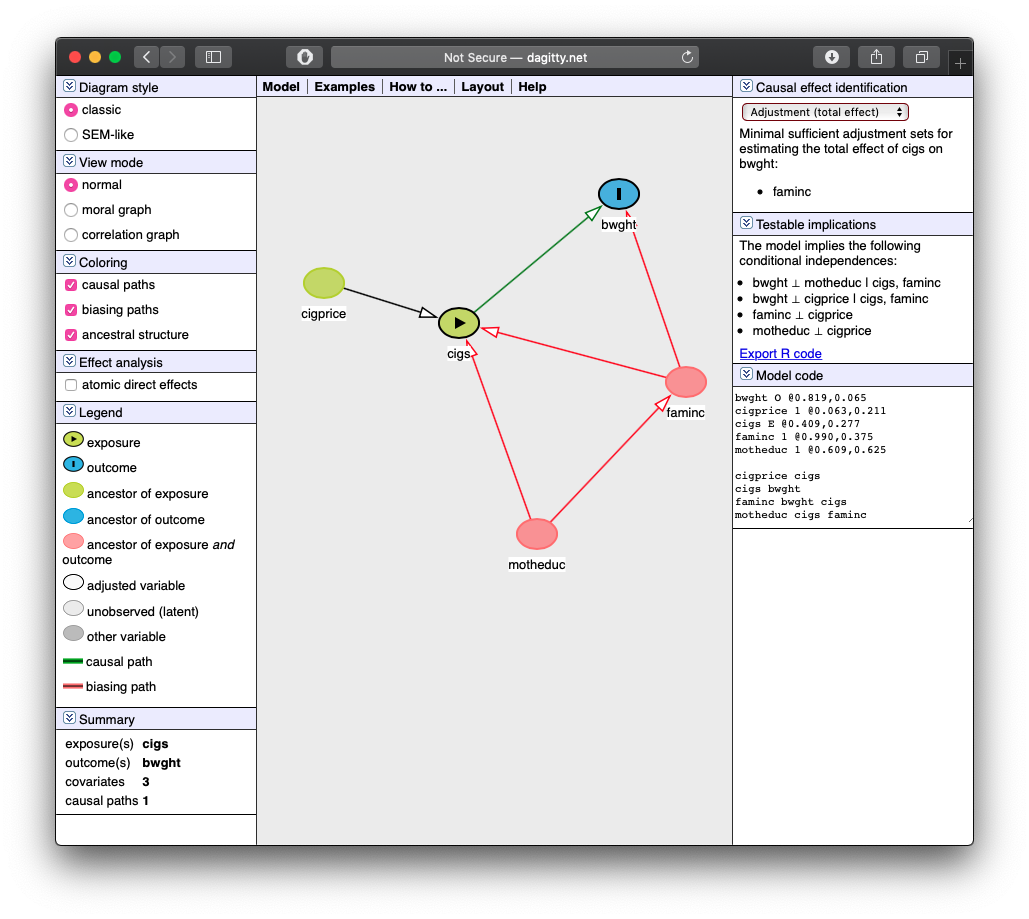
\includegraphics{../images/4dagitty.png}

See the middle box on the right on dagitty:

\begin{enumerate}
\def\labelenumi{\arabic{enumi}.}
\item
  \(bwght \perp price \, | \, cigs, inc\): birthweight is independent of
  price, controlling for cigarettes and income
\item
  \(bwght \perp educ \, | \, cigs, inc\): birthweight is independent of
  education, controlling for cigarettes and income
\item
  \(inc \perp price\): income is independent of price
\item
  \(price \perp educ\): cigarette price is independent of education
\end{enumerate}

\begin{Shaded}
\begin{Highlighting}[]
\CommentTok{\# note you can do it in R with the dagitty package\textquotesingle{}s command,}
\CommentTok{\# impliedConditionalIndependencies()}

\CommentTok{\# ensure dagitty is loaded}
\FunctionTok{library}\NormalTok{(dagitty)}

\CommentTok{\# save the dag (before plotted, so the part inside dagify() command}
\CommentTok{\# that I created in the question}
\NormalTok{dag }\OtherTok{\textless{}{-}} \FunctionTok{dagify}\NormalTok{(bwght }\SpecialCharTok{\textasciitilde{}}\NormalTok{ cigs }\SpecialCharTok{+}\NormalTok{ inc,}
\NormalTok{       cigs }\SpecialCharTok{\textasciitilde{}}\NormalTok{ price }\SpecialCharTok{+}\NormalTok{ educ }\SpecialCharTok{+}\NormalTok{ inc,}
\NormalTok{       inc }\SpecialCharTok{\textasciitilde{}}\NormalTok{ educ,}
       \AttributeTok{exposure =} \StringTok{"cigs"}\NormalTok{,}
       \AttributeTok{outcome =} \StringTok{"bwght"}\NormalTok{)}

\CommentTok{\# now pipe it into command}
\NormalTok{dag }\SpecialCharTok{\%\textgreater{}\%} \FunctionTok{impliedConditionalIndependencies}\NormalTok{()}
\end{Highlighting}
\end{Shaded}

\begin{verbatim}
## bwgh _||_ educ | cigs, inc
## bwgh _||_ pric | cigs, inc
## educ _||_ pric
## inc _||_ pric
\end{verbatim}

\begin{center}\rule{0.5\linewidth}{0.5pt}\end{center}

\hypertarget{part-c-2}{%
\subsubsection{Part C}\label{part-c-2}}

Test each implication given to you by \texttt{dagitty.}

\begin{itemize}
\tightlist
\item
  For independencies, e.g.~\((x \perp y)\): run a regression of \(y\) on
  \(x\).
\item
  For \emph{conditional} independencies, e.g.~\((x \perp y | z, a)\):
  run a regression of \(y\) on \(x, z, a\).
\end{itemize}

For each, test against the null hypothesis that the relevant coefficient
\((\beta_1) =0\) (i.e.~\(x\) and \(y\) are indeed independent).

Does this causal model hold up well?

\begin{center}\rule{0.5\linewidth}{0.5pt}\end{center}

\hypertarget{implication-1}{%
\paragraph{Implication 1:}\label{implication-1}}

If we run a regression of \texttt{bwght} on \texttt{cigprice}, including
\texttt{cigs} and \texttt{faminc} as controls, there should not not be a
statistically significant coefficient on \texttt{cigprice} (i.e.~there
is no relationship between \texttt{cigprice} and \texttt{bwght} holding
\texttt{cigs} and\texttt{faminc} constant):

\begin{Shaded}
\begin{Highlighting}[]
\FunctionTok{lm}\NormalTok{(bwght }\SpecialCharTok{\textasciitilde{}}\NormalTok{ cigprice }\SpecialCharTok{+}\NormalTok{  cigs }\SpecialCharTok{+}\NormalTok{ faminc, }\AttributeTok{data =}\NormalTok{ bwght) }\SpecialCharTok{\%\textgreater{}\%} \FunctionTok{summary}\NormalTok{()}
\end{Highlighting}
\end{Shaded}

\begin{verbatim}
## 
## Call:
## lm(formula = bwght ~ cigprice + cigs + faminc, data = bwght)
## 
## Residuals:
##     Min      1Q  Median      3Q     Max 
## -95.746 -11.516   0.784  13.175 149.956 
## 
## Coefficients:
##              Estimate Std. Error t value Pr(>|t|)    
## (Intercept) 106.02164    6.88671  15.395  < 2e-16 ***
## cigprice      0.08499    0.05282   1.609   0.1078    
## cigs         -0.46735    0.09156  -5.104 3.78e-07 ***
## faminc        0.08811    0.02931   3.006   0.0027 ** 
## ---
## Signif. codes:  0 '***' 0.001 '**' 0.01 '*' 0.05 '.' 0.1 ' ' 1
## 
## Residual standard error: 20.05 on 1384 degrees of freedom
## Multiple R-squared:  0.03162,    Adjusted R-squared:  0.02952 
## F-statistic: 15.06 on 3 and 1384 DF,  p-value: 1.193e-09
\end{verbatim}

The coefficient on \texttt{cigprice} is small and not statistically
significant. This implication holds up well.

\hypertarget{implication-2}{%
\paragraph{Implication 2:}\label{implication-2}}

If we run a regression of \texttt{bwght} on \texttt{motheduc}, including
\texttt{cigs} and \texttt{faminc} as controls, there should not not be a
statistically significant coefficient on \texttt{cigprice} (i.e.~there
is no relationship between \texttt{motheduc} and \texttt{bwght} holding
\texttt{cigs} and\texttt{faminc} constant):

\begin{Shaded}
\begin{Highlighting}[]
\FunctionTok{lm}\NormalTok{(bwght }\SpecialCharTok{\textasciitilde{}}\NormalTok{ motheduc }\SpecialCharTok{+}\NormalTok{ cigs }\SpecialCharTok{+}\NormalTok{ faminc, }\AttributeTok{data =}\NormalTok{ bwght) }\SpecialCharTok{\%\textgreater{}\%} \FunctionTok{summary}\NormalTok{()}
\end{Highlighting}
\end{Shaded}

\begin{verbatim}
## 
## Call:
## lm(formula = bwght ~ motheduc + cigs + faminc, data = bwght)
## 
## Residuals:
##     Min      1Q  Median      3Q     Max 
## -96.064 -11.585   0.668  13.154 150.078 
## 
## Coefficients:
##              Estimate Std. Error t value Pr(>|t|)    
## (Intercept) 116.83485    3.13778  37.235  < 2e-16 ***
## motheduc      0.01426    0.25799   0.055   0.9559    
## cigs         -0.46335    0.09275  -4.996 6.61e-07 ***
## faminc        0.09147    0.03246   2.818   0.0049 ** 
## ---
## Signif. codes:  0 '***' 0.001 '**' 0.01 '*' 0.05 '.' 0.1 ' ' 1
## 
## Residual standard error: 20.08 on 1383 degrees of freedom
##   (1 observation deleted due to missingness)
## Multiple R-squared:  0.02977,    Adjusted R-squared:  0.02767 
## F-statistic: 14.15 on 3 and 1383 DF,  p-value: 4.385e-09
\end{verbatim}

\hypertarget{implication-3}{%
\paragraph{Implication 3:}\label{implication-3}}

The model implies simply that there is no significant correlation
between \texttt{faminc} and \texttt{cigprice}

\begin{Shaded}
\begin{Highlighting}[]
\NormalTok{bwght }\SpecialCharTok{\%\textgreater{}\%}
  \FunctionTok{select}\NormalTok{(faminc, cigprice) }\SpecialCharTok{\%\textgreater{}\%}
  \FunctionTok{cor}\NormalTok{()}
\end{Highlighting}
\end{Shaded}

\begin{verbatim}
##              faminc   cigprice
## faminc   1.00000000 0.09545581
## cigprice 0.09545581 1.00000000
\end{verbatim}

There is a fairly weak correlation. This implication mostly holds up.

\hypertarget{implication-4}{%
\paragraph{Implication 4:}\label{implication-4}}

The model implies simply that there is no significant correlation
between \texttt{cigprice} and \texttt{motheduc}

\begin{Shaded}
\begin{Highlighting}[]
\NormalTok{bwght }\SpecialCharTok{\%\textgreater{}\%}
  \FunctionTok{select}\NormalTok{(cigprice, motheduc) }\SpecialCharTok{\%\textgreater{}\%}
  \FunctionTok{cor}\NormalTok{(}\AttributeTok{use =} \StringTok{"pairwise.complete.obs"}\NormalTok{)}
\end{Highlighting}
\end{Shaded}

\begin{verbatim}
##            cigprice   motheduc
## cigprice 1.00000000 0.07086587
## motheduc 0.07086587 1.00000000
\end{verbatim}

This is an even weaker correlation. This implication seems to holds up.

\begin{center}\rule{0.5\linewidth}{0.5pt}\end{center}

\hypertarget{part-d-1}{%
\subsubsection{Part D}\label{part-d-1}}

\textbf{List \emph{all} of the possible pathways from \texttt{cigs} to
\texttt{bwght}. Which are ``front-doors'' and which are ``back-doors?''
Are any blocked by colliders?}

\begin{center}\rule{0.5\linewidth}{0.5pt}\end{center}

\begin{enumerate}
\def\labelenumi{\arabic{enumi}.}
\tightlist
\item
  \(cigs \rightarrow bwght\) (causal, front door)
\item
  \(cigs \leftarrow faminc \rightarrow bwght\) (non-causal, back door)
\item
  \(cibs \leftarrow motheduc \rightarrow faminc \rightarrow bwght\)
  (non-causal, back door)
\end{enumerate}

There are no colliders on any path.

\begin{Shaded}
\begin{Highlighting}[]
\CommentTok{\# we can also get this from R in ggdag}
\CommentTok{\# using ggdag\_paths()}

\FunctionTok{library}\NormalTok{(ggdag)}

\NormalTok{dag }\SpecialCharTok{\%\textgreater{}\%}
  \FunctionTok{ggdag\_paths}\NormalTok{()}\SpecialCharTok{+}
  \FunctionTok{theme\_dag}\NormalTok{()}
\end{Highlighting}
\end{Shaded}

\hypertarget{section}{%
\subsection{\texorpdfstring{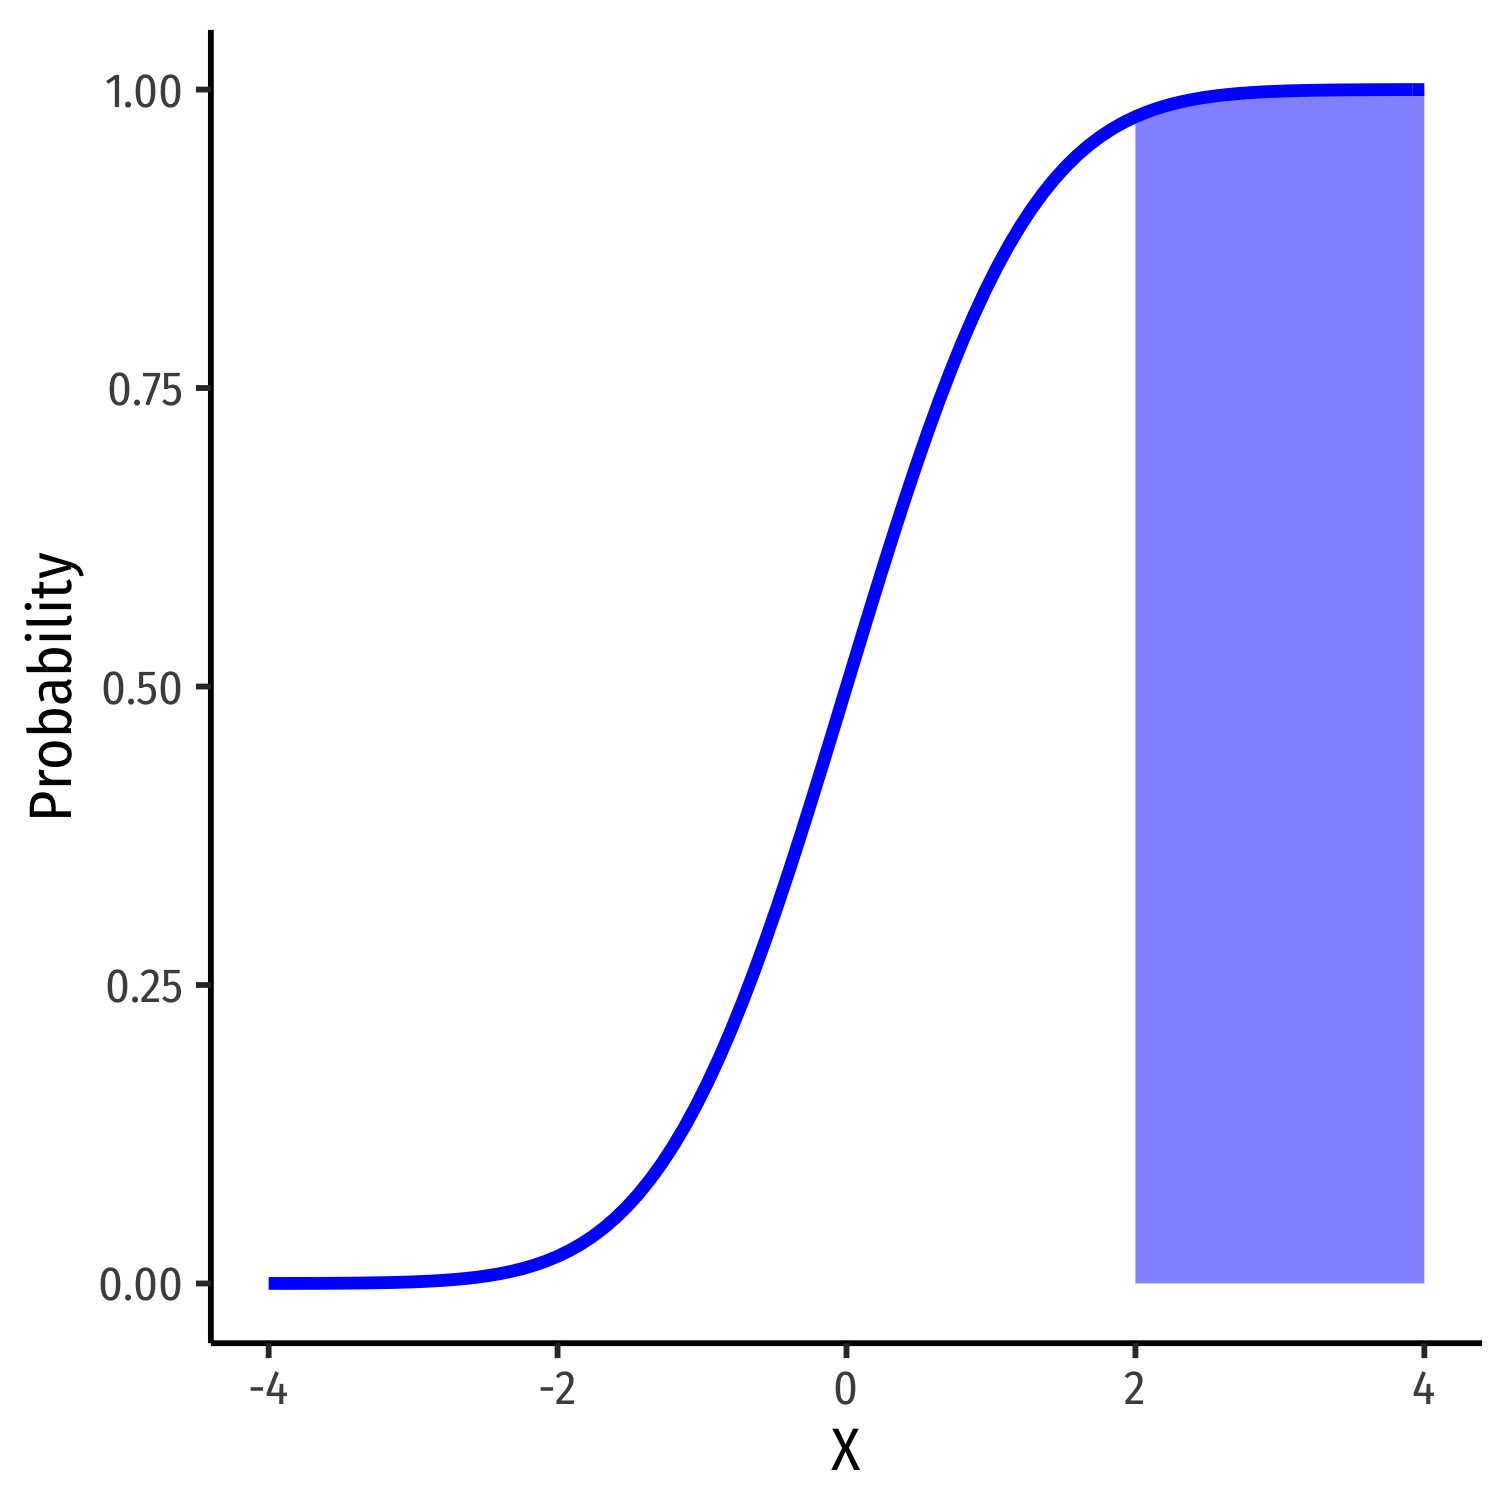
\includegraphics[width=0.8\linewidth]{04-problem-set-answers-pdf_files/figure-latex/unnamed-chunk-13-1}}{}}\label{section}}

\hypertarget{part-e}{%
\subsubsection{Part E}\label{part-e}}

\textbf{What is the minimal sufficient set of variables we need to
control for in order to causally identify the effect of \texttt{cigs} on
\texttt{bwght}?}

\begin{center}\rule{0.5\linewidth}{0.5pt}\end{center}

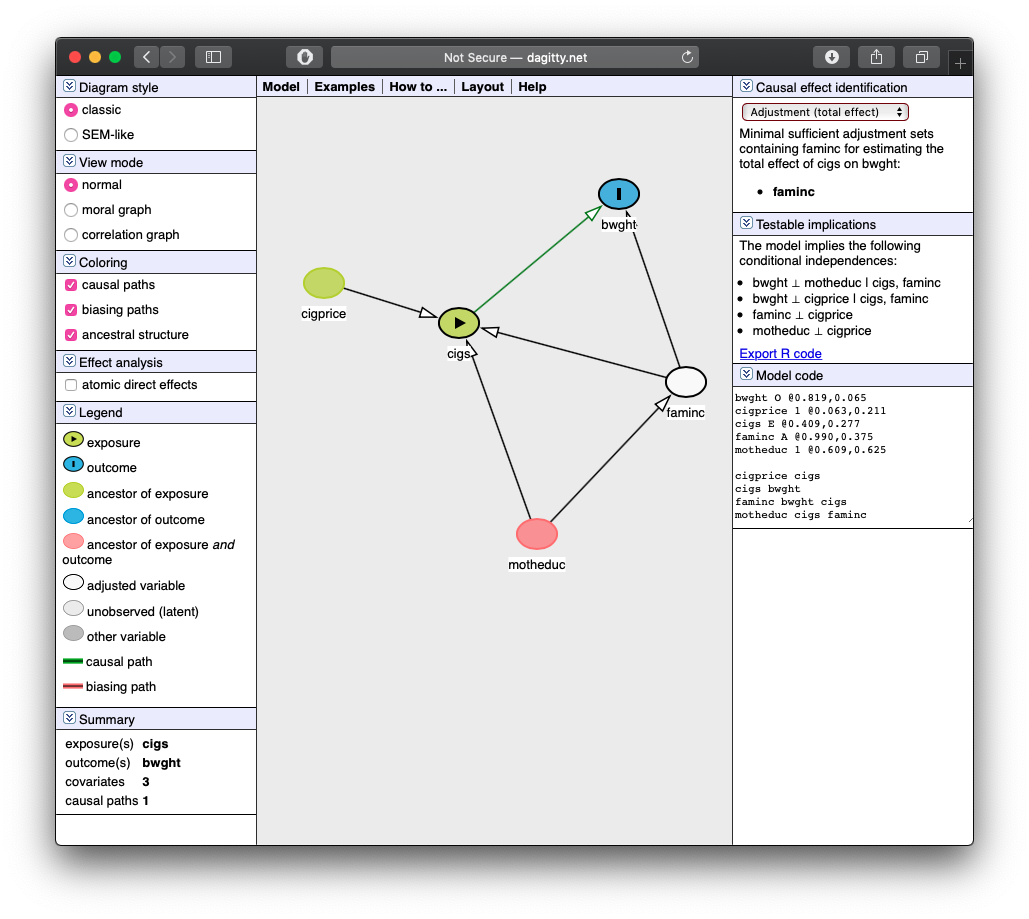
\includegraphics{../images/7dagitty.png}

We simply need to control for \texttt{faminc}. This blocks the back door
for both path 2 and path 3.

\begin{Shaded}
\begin{Highlighting}[]
\CommentTok{\# we can also get this from R in ggdag}
\CommentTok{\# using ggdag\_adjustment\_set()}

\FunctionTok{library}\NormalTok{(ggdag)}

\NormalTok{dag }\SpecialCharTok{\%\textgreater{}\%}
  \FunctionTok{ggdag\_adjustment\_set}\NormalTok{(}\AttributeTok{shadow =}\NormalTok{ T)}\SpecialCharTok{+}
  \FunctionTok{theme\_dag}\NormalTok{()}
\end{Highlighting}
\end{Shaded}

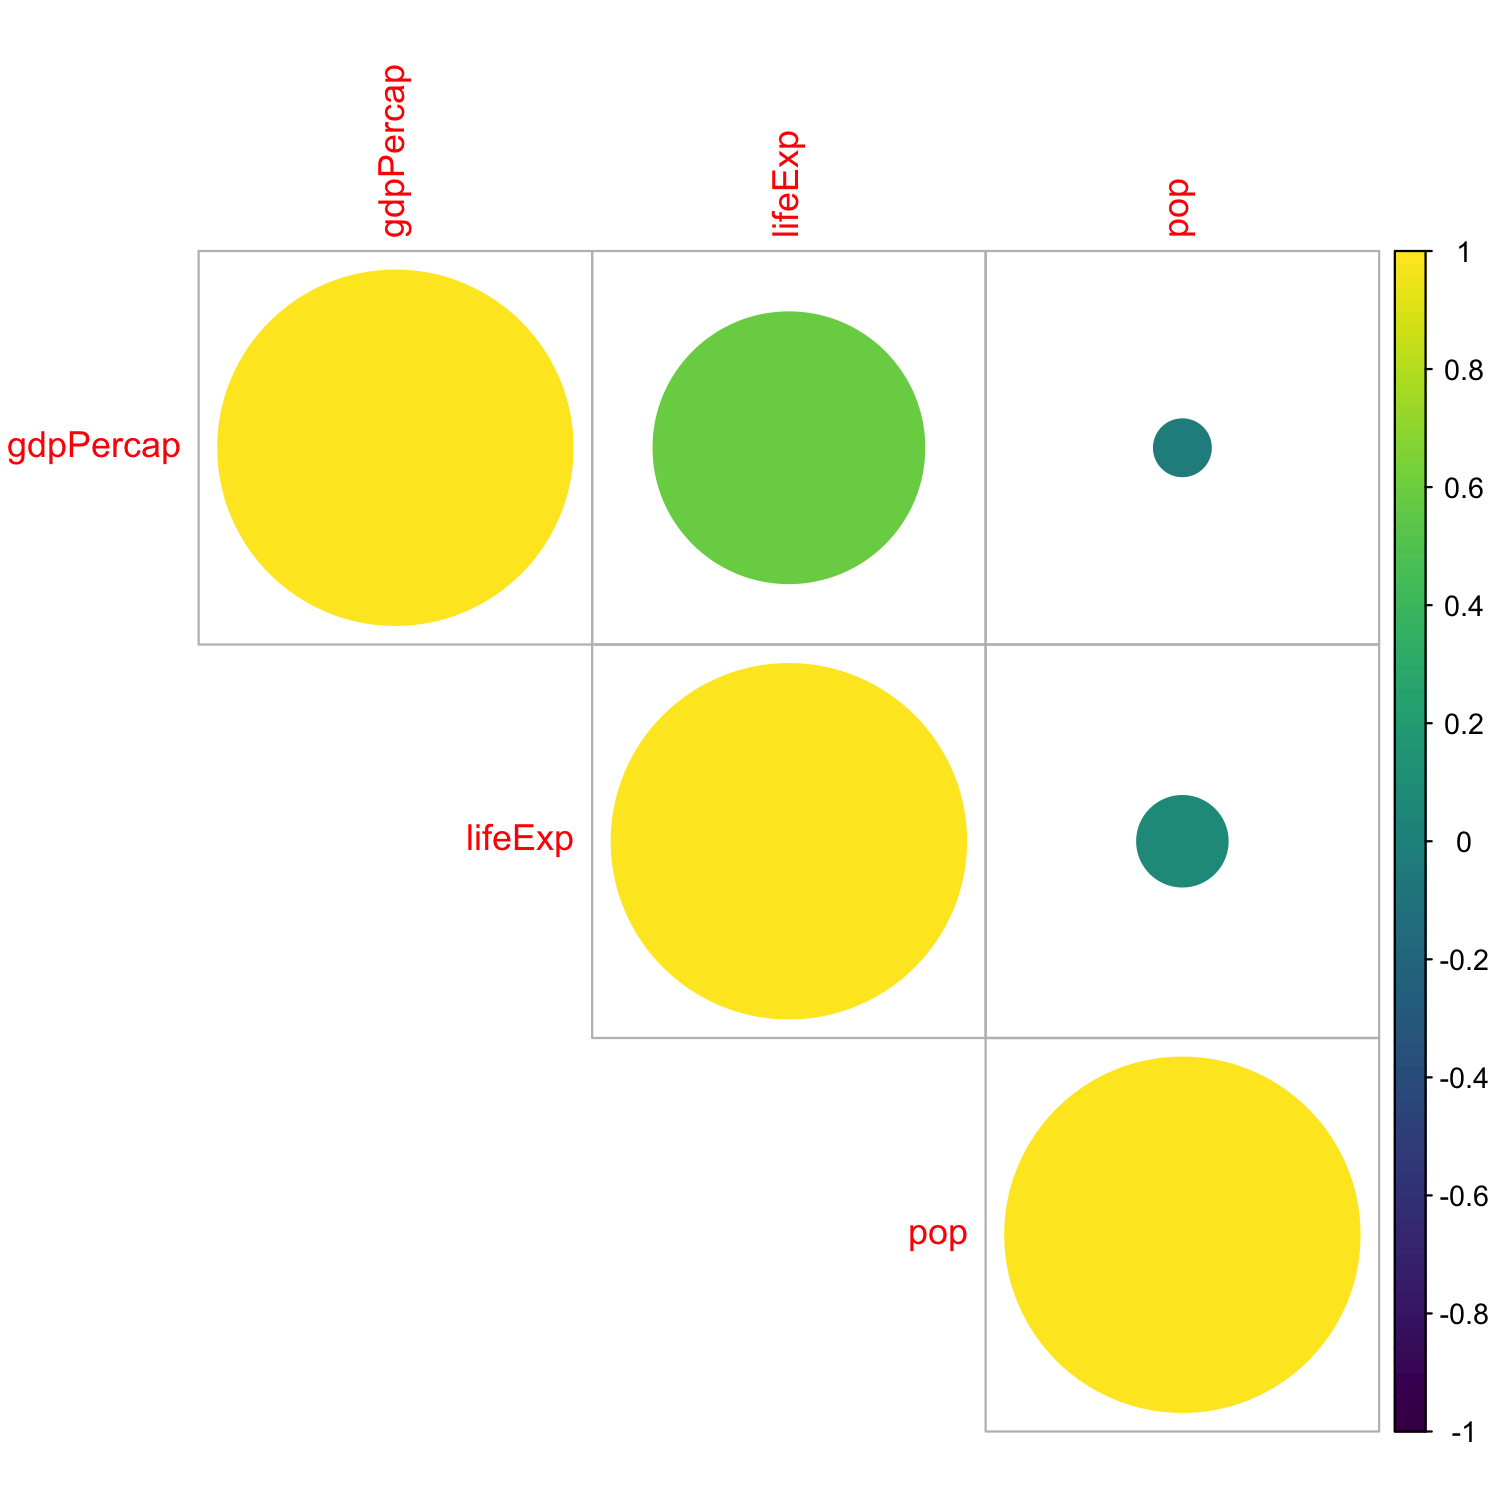
\includegraphics[width=0.8\linewidth]{04-problem-set-answers-pdf_files/figure-latex/unnamed-chunk-14-1}

\begin{center}\rule{0.5\linewidth}{0.5pt}\end{center}

\hypertarget{part-f}{%
\subsubsection{Part F}\label{part-f}}

\textbf{Estimate the causal effect by running the appropriate
regression.}

\textbf{FYI, on \texttt{dagitty.net}, you can change a variable on the
diagram to be ``\emph{adjusted}'' (controlled for) by clicking it and
then hitting the \texttt{A} key.}

\begin{center}\rule{0.5\linewidth}{0.5pt}\end{center}

We need to control only for \texttt{faminc}, so we put it into the
regression to estimate:

\[bwght_i=\beta_0+\beta_1 \, cigs_i+\beta_2 \,faminc_i\]

\begin{Shaded}
\begin{Highlighting}[]
\FunctionTok{lm}\NormalTok{(bwght }\SpecialCharTok{\textasciitilde{}}\NormalTok{ cigs }\SpecialCharTok{+}\NormalTok{ faminc, }\AttributeTok{data =}\NormalTok{ bwght) }\SpecialCharTok{\%\textgreater{}\%} \FunctionTok{summary}\NormalTok{()}
\end{Highlighting}
\end{Shaded}

\begin{verbatim}
## 
## Call:
## lm(formula = bwght ~ cigs + faminc, data = bwght)
## 
## Residuals:
##     Min      1Q  Median      3Q     Max 
## -96.061 -11.543   0.638  13.126 150.083 
## 
## Coefficients:
##              Estimate Std. Error t value Pr(>|t|)    
## (Intercept) 116.97413    1.04898 111.512  < 2e-16 ***
## cigs         -0.46341    0.09158  -5.060 4.75e-07 ***
## faminc        0.09276    0.02919   3.178  0.00151 ** 
## ---
## Signif. codes:  0 '***' 0.001 '**' 0.01 '*' 0.05 '.' 0.1 ' ' 1
## 
## Residual standard error: 20.06 on 1385 degrees of freedom
## Multiple R-squared:  0.0298, Adjusted R-squared:  0.0284 
## F-statistic: 21.27 on 2 and 1385 DF,  p-value: 7.942e-10
\end{verbatim}

Controlling for income, each cigarette smoked while pregant will cause
the birthweight to decrease by 0.46 ounces.

\begin{center}\rule{0.5\linewidth}{0.5pt}\end{center}

\hypertarget{part-g}{%
\subsubsection{Part G}\label{part-g}}

\textbf{We saw some effect between \texttt{faminc} and
\texttt{cigprice}. Perhaps there are unobserved factors (such as the
economy's performance) that affect both. Add an unobserved factor
\texttt{u1} to your \texttt{dagitty} model.}

\textbf{FYI, on \texttt{dagitty.net}, you can make a variable be
``\emph{unobserved}'' by double-clicking it and then hitting the
\texttt{U} key.}

\begin{center}\rule{0.5\linewidth}{0.5pt}\end{center}

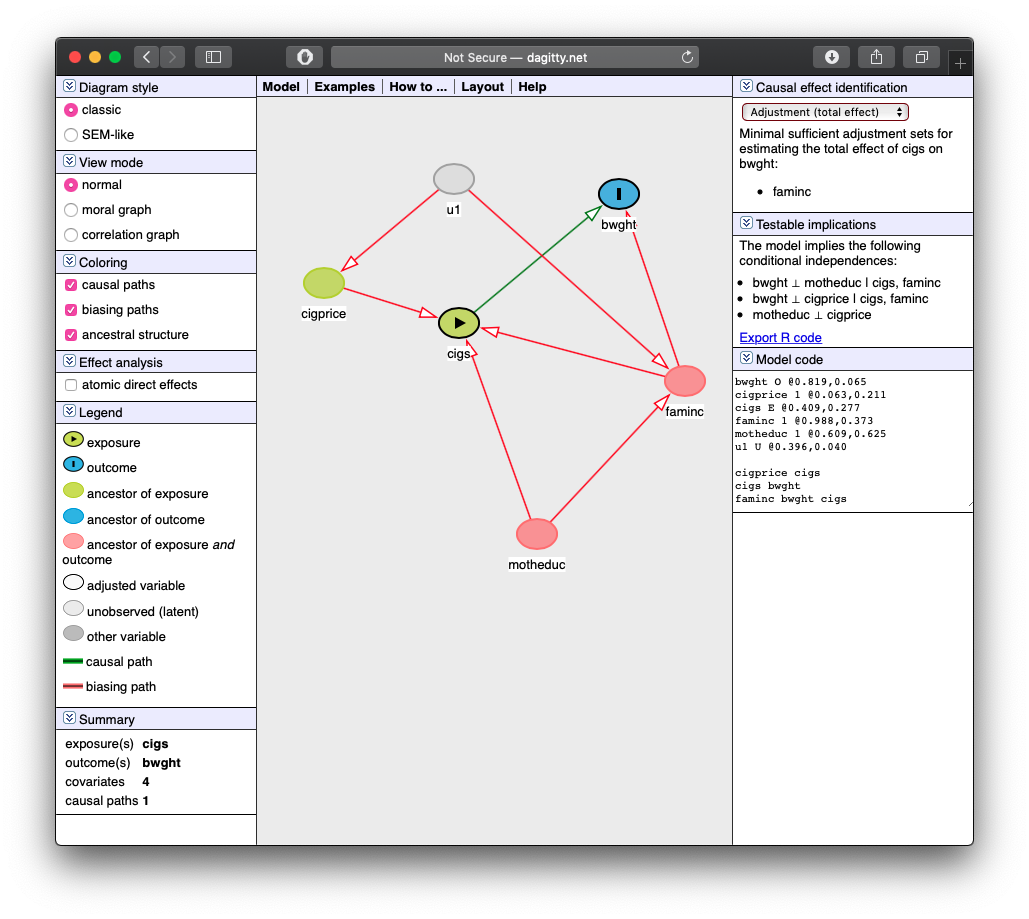
\includegraphics{../images/9dagitty.png}

\begin{Shaded}
\begin{Highlighting}[]
\CommentTok{\# write your code here}
\end{Highlighting}
\end{Shaded}

\begin{center}\rule{0.5\linewidth}{0.5pt}\end{center}

\hypertarget{part-h}{%
\subsubsection{Part H}\label{part-h}}

\textbf{Perhaps our model is poorly specified. Maybe \texttt{motheduc}
actually has a causal effect on \texttt{bwght}? Tweak your model from
Question 9 on \texttt{dagitty} to add this potential relationship. What
testable implications does this new model imply?}

\begin{center}\rule{0.5\linewidth}{0.5pt}\end{center}

See the middle box on the right on dagitty:

\begin{enumerate}
\def\labelenumi{\arabic{enumi}.}
\item
  \(bwght \perp price \, | \, cigs, inc, educ\): birthweight is
  independent of price, controlling for cigarettes, income, and
  education
\item
  \(price \perp educ\): cigarette price is independent of education
\item
  \(inc \perp price\): income is independent of cigarette price
\end{enumerate}

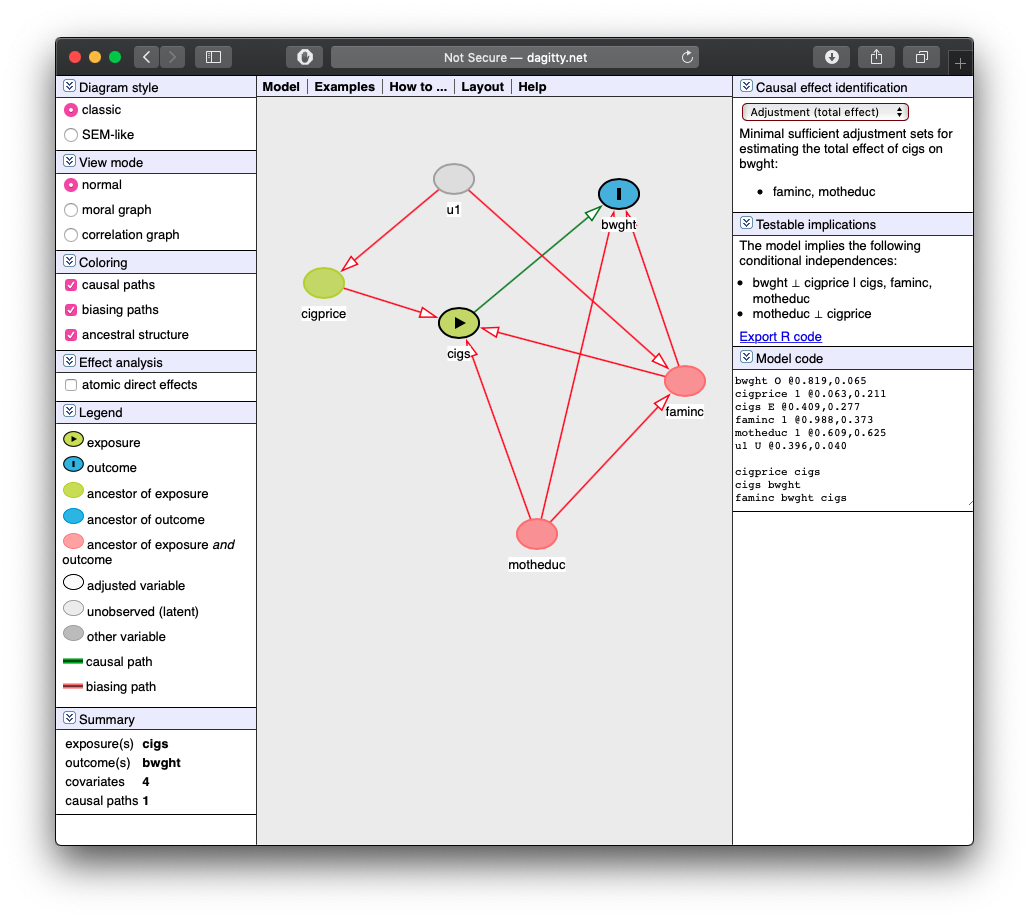
\includegraphics{../images/10dagitty.png}

\begin{Shaded}
\begin{Highlighting}[]
\CommentTok{\# we can also do this in R}

\CommentTok{\# update the DAG}

\NormalTok{dag2 }\OtherTok{\textless{}{-}} \FunctionTok{dagify}\NormalTok{(bwght }\SpecialCharTok{\textasciitilde{}}\NormalTok{ cigs }\SpecialCharTok{+}\NormalTok{ inc }\SpecialCharTok{+}\NormalTok{ educ, }\CommentTok{\#\textless{}\textless{} add educ}
\NormalTok{       cigs }\SpecialCharTok{\textasciitilde{}}\NormalTok{ price }\SpecialCharTok{+}\NormalTok{ educ }\SpecialCharTok{+}\NormalTok{ inc,}
\NormalTok{       inc }\SpecialCharTok{\textasciitilde{}}\NormalTok{ educ,}
       \AttributeTok{exposure =} \StringTok{"cigs"}\NormalTok{,}
       \AttributeTok{outcome =} \StringTok{"bwght"}\NormalTok{)}

\CommentTok{\# now pipe it into command}
\NormalTok{dag2 }\SpecialCharTok{\%\textgreater{}\%} \FunctionTok{impliedConditionalIndependencies}\NormalTok{()}
\end{Highlighting}
\end{Shaded}

\begin{verbatim}
## bwgh _||_ pric | cigs, educ, inc
## educ _||_ pric
## inc _||_ pric
\end{verbatim}

\begin{center}\rule{0.5\linewidth}{0.5pt}\end{center}

\hypertarget{part-i}{%
\subsubsection{Part I}\label{part-i}}

\textbf{Test these implications appropriately, like you did in Part C.
Does this model hold up well?}

\begin{center}\rule{0.5\linewidth}{0.5pt}\end{center}

\hypertarget{implication-1-1}{%
\paragraph{Implication 1:}\label{implication-1-1}}

If we run a regression of \texttt{bwght} on \texttt{cigprice}, including
\texttt{cigs}, \texttt{faminc}, and \texttt{motheduc} as controls, there
should not not be a statistically significant coefficient on
\texttt{cigprice} (i.e.~there is no relationship between
\texttt{cigprice} and \texttt{bwght} holding
\texttt{cigs},\texttt{faminc}, and \texttt{motheduc} constant):

\begin{Shaded}
\begin{Highlighting}[]
\FunctionTok{lm}\NormalTok{(bwght }\SpecialCharTok{\textasciitilde{}}\NormalTok{ cigprice }\SpecialCharTok{+}\NormalTok{ cigs }\SpecialCharTok{+}\NormalTok{ faminc }\SpecialCharTok{+}\NormalTok{ motheduc, }\AttributeTok{data =}\NormalTok{ bwght) }\SpecialCharTok{\%\textgreater{}\%} \FunctionTok{summary}\NormalTok{()}
\end{Highlighting}
\end{Shaded}

\begin{verbatim}
## 
## Call:
## lm(formula = bwght ~ cigprice + cigs + faminc + motheduc, data = bwght)
## 
## Residuals:
##     Min      1Q  Median      3Q     Max 
## -95.760 -11.519   0.803  13.175 149.954 
## 
## Coefficients:
##               Estimate Std. Error t value Pr(>|t|)    
## (Intercept)  1.061e+02  7.407e+00  14.321  < 2e-16 ***
## cigprice     8.478e-02  5.288e-02   1.603  0.10912    
## cigs        -4.681e-01  9.274e-02  -5.047 5.08e-07 ***
## faminc       8.765e-02  3.253e-02   2.694  0.00714 ** 
## motheduc    -4.448e-04  2.580e-01  -0.002  0.99862    
## ---
## Signif. codes:  0 '***' 0.001 '**' 0.01 '*' 0.05 '.' 0.1 ' ' 1
## 
## Residual standard error: 20.06 on 1382 degrees of freedom
##   (1 observation deleted due to missingness)
## Multiple R-squared:  0.03158,    Adjusted R-squared:  0.02877 
## F-statistic: 11.26 on 4 and 1382 DF,  p-value: 5.368e-09
\end{verbatim}

The coefficient on \texttt{cigprice} is small and not statistically
significant. This implication holds up well.

\hypertarget{implication-2-1}{%
\paragraph{Implication 2:}\label{implication-2-1}}

This is the same as implication 3 from Part C. Again, this holds up
reasonably well.

\hypertarget{implication-3-1}{%
\paragraph{Implication 3:}\label{implication-3-1}}

This is the same as implication 4 from Part C. Again, this holds up
reasonably well.

\begin{center}\rule{0.5\linewidth}{0.5pt}\end{center}

\hypertarget{part-j}{%
\subsubsection{Part J}\label{part-j}}

\textbf{Under this new causal model, list \emph{all} of the possible
pathways from \texttt{cigs} to \texttt{bwght}. Which are ``front-doors''
and which are ``back-doors?'' Are any blocked by colliders?}

\begin{center}\rule{0.5\linewidth}{0.5pt}\end{center}

\begin{enumerate}
\def\labelenumi{\arabic{enumi}.}
\tightlist
\item
  \(cigs \rightarrow bwght\) (causal, front door)
\item
  \(cigs \leftarrow faminc \rightarrow bwght\) (non-causal, back door)
\item
  \(cigs \leftarrow cigprice \leftarrow u1 \rightarrow faminc \rightarrow bwght\)
  (non-causal, back door)
\item
  \(cigs \leftarrow motheduc \rightarrow bwght\) (non-causal, back door)
\item
  \(cigs \leftarrow motheduc \rightarrow faminc \rightarrow bwght\)
  (non-causal, back door)
\end{enumerate}

\begin{Shaded}
\begin{Highlighting}[]
\CommentTok{\# we can also get this from R in ggdag}
\CommentTok{\# using ggdag\_paths()}

\NormalTok{dag2 }\SpecialCharTok{\%\textgreater{}\%}
  \FunctionTok{ggdag\_paths}\NormalTok{()}\SpecialCharTok{+}
  \FunctionTok{theme\_dag}\NormalTok{()}
\end{Highlighting}
\end{Shaded}

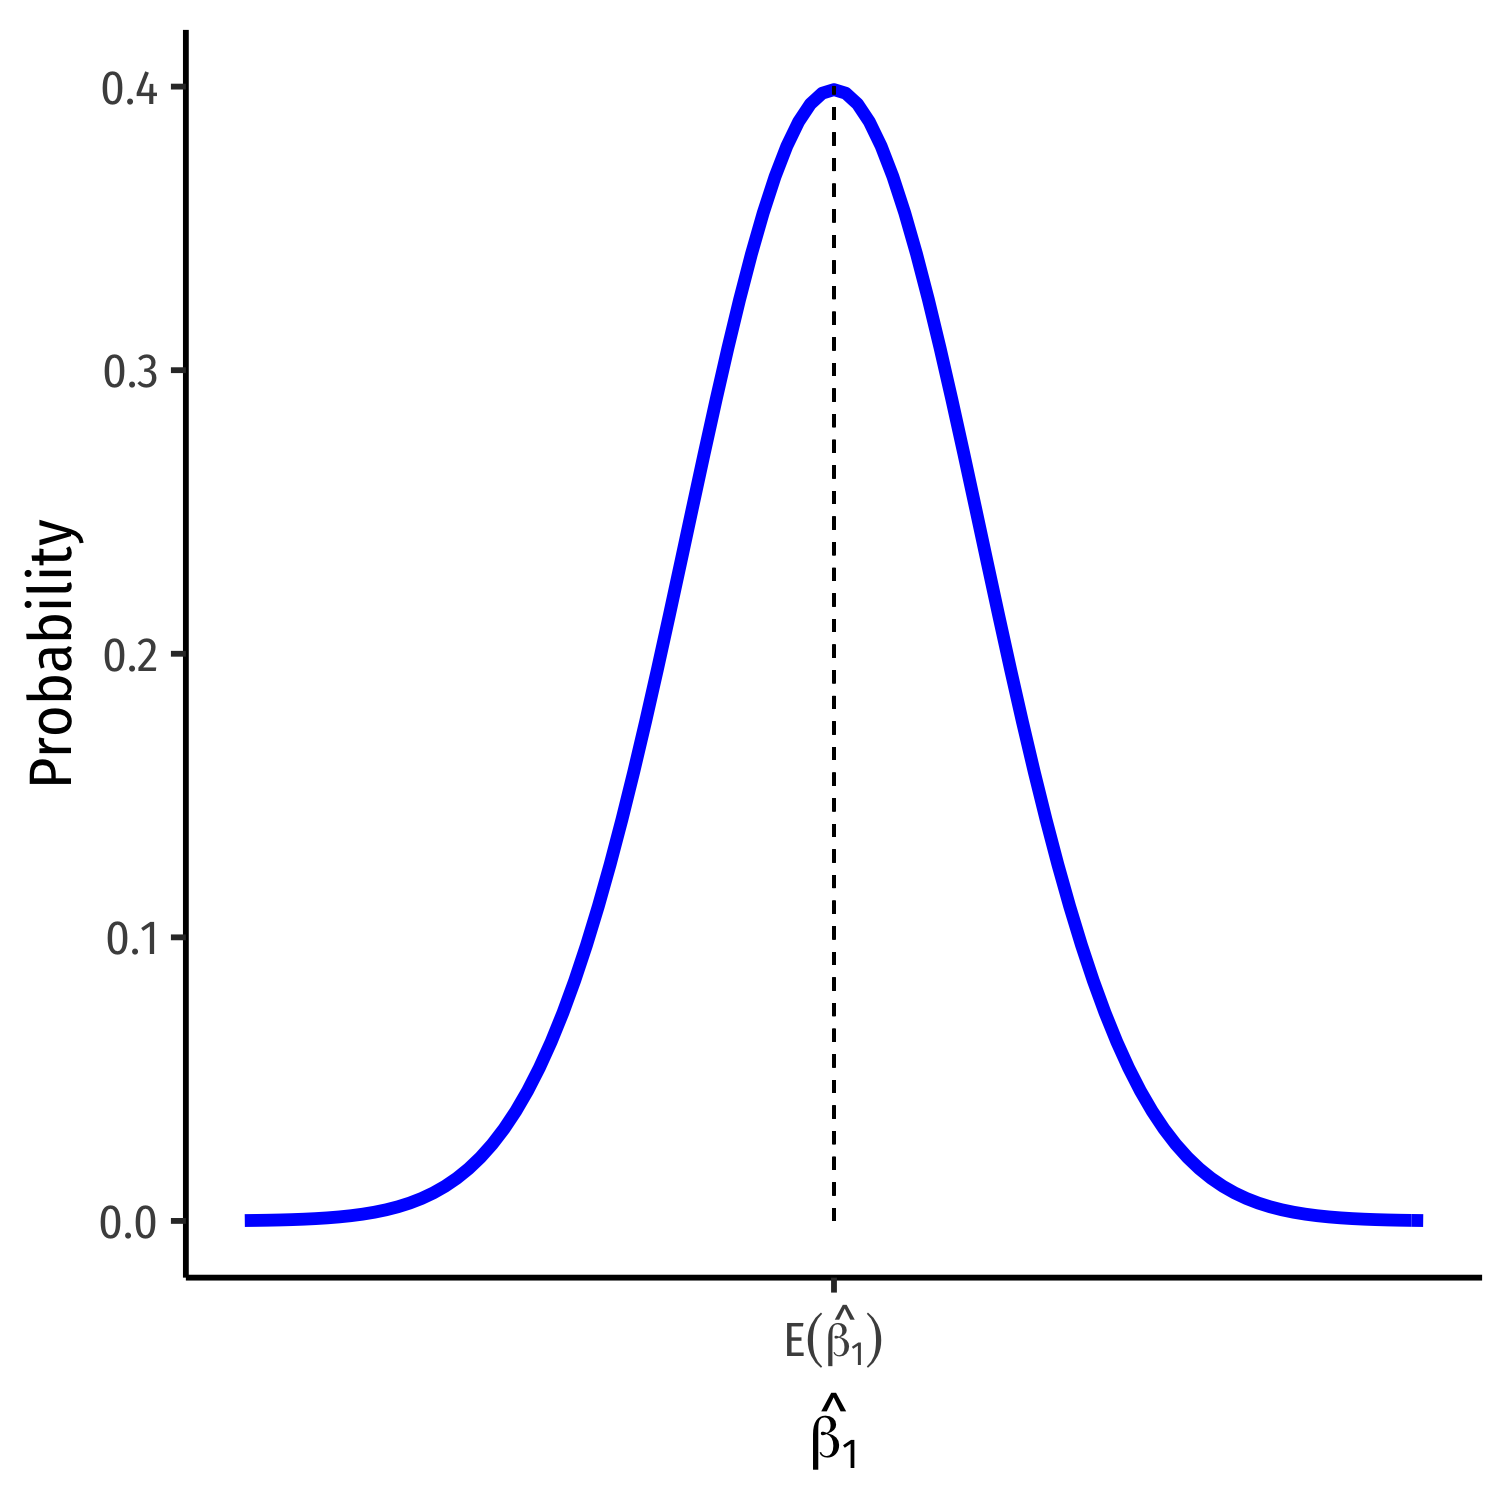
\includegraphics[width=0.8\linewidth]{04-problem-set-answers-pdf_files/figure-latex/unnamed-chunk-19-1}

\begin{center}\rule{0.5\linewidth}{0.5pt}\end{center}

\hypertarget{part-k}{%
\subsubsection{Part K}\label{part-k}}

\textbf{Under this new causal model, what is the minimal sufficient set
of variables we need to control in order to causally identify the effect
of \texttt{cigs} on \texttt{bwght}?}

\begin{center}\rule{0.5\linewidth}{0.5pt}\end{center}

We need to control for \texttt{faminc} and \texttt{motheduc}. This
blocks the back door for paths 2, 3, 4, and 5.

\begin{Shaded}
\begin{Highlighting}[]
\CommentTok{\# we can also get this from R in ggdag}
\CommentTok{\# using ggdag\_adjustment\_set()}

\NormalTok{dag2 }\SpecialCharTok{\%\textgreater{}\%}
  \FunctionTok{ggdag\_adjustment\_set}\NormalTok{(}\AttributeTok{shadow =}\NormalTok{ T)}\SpecialCharTok{+}
  \FunctionTok{theme\_dag}\NormalTok{()}
\end{Highlighting}
\end{Shaded}

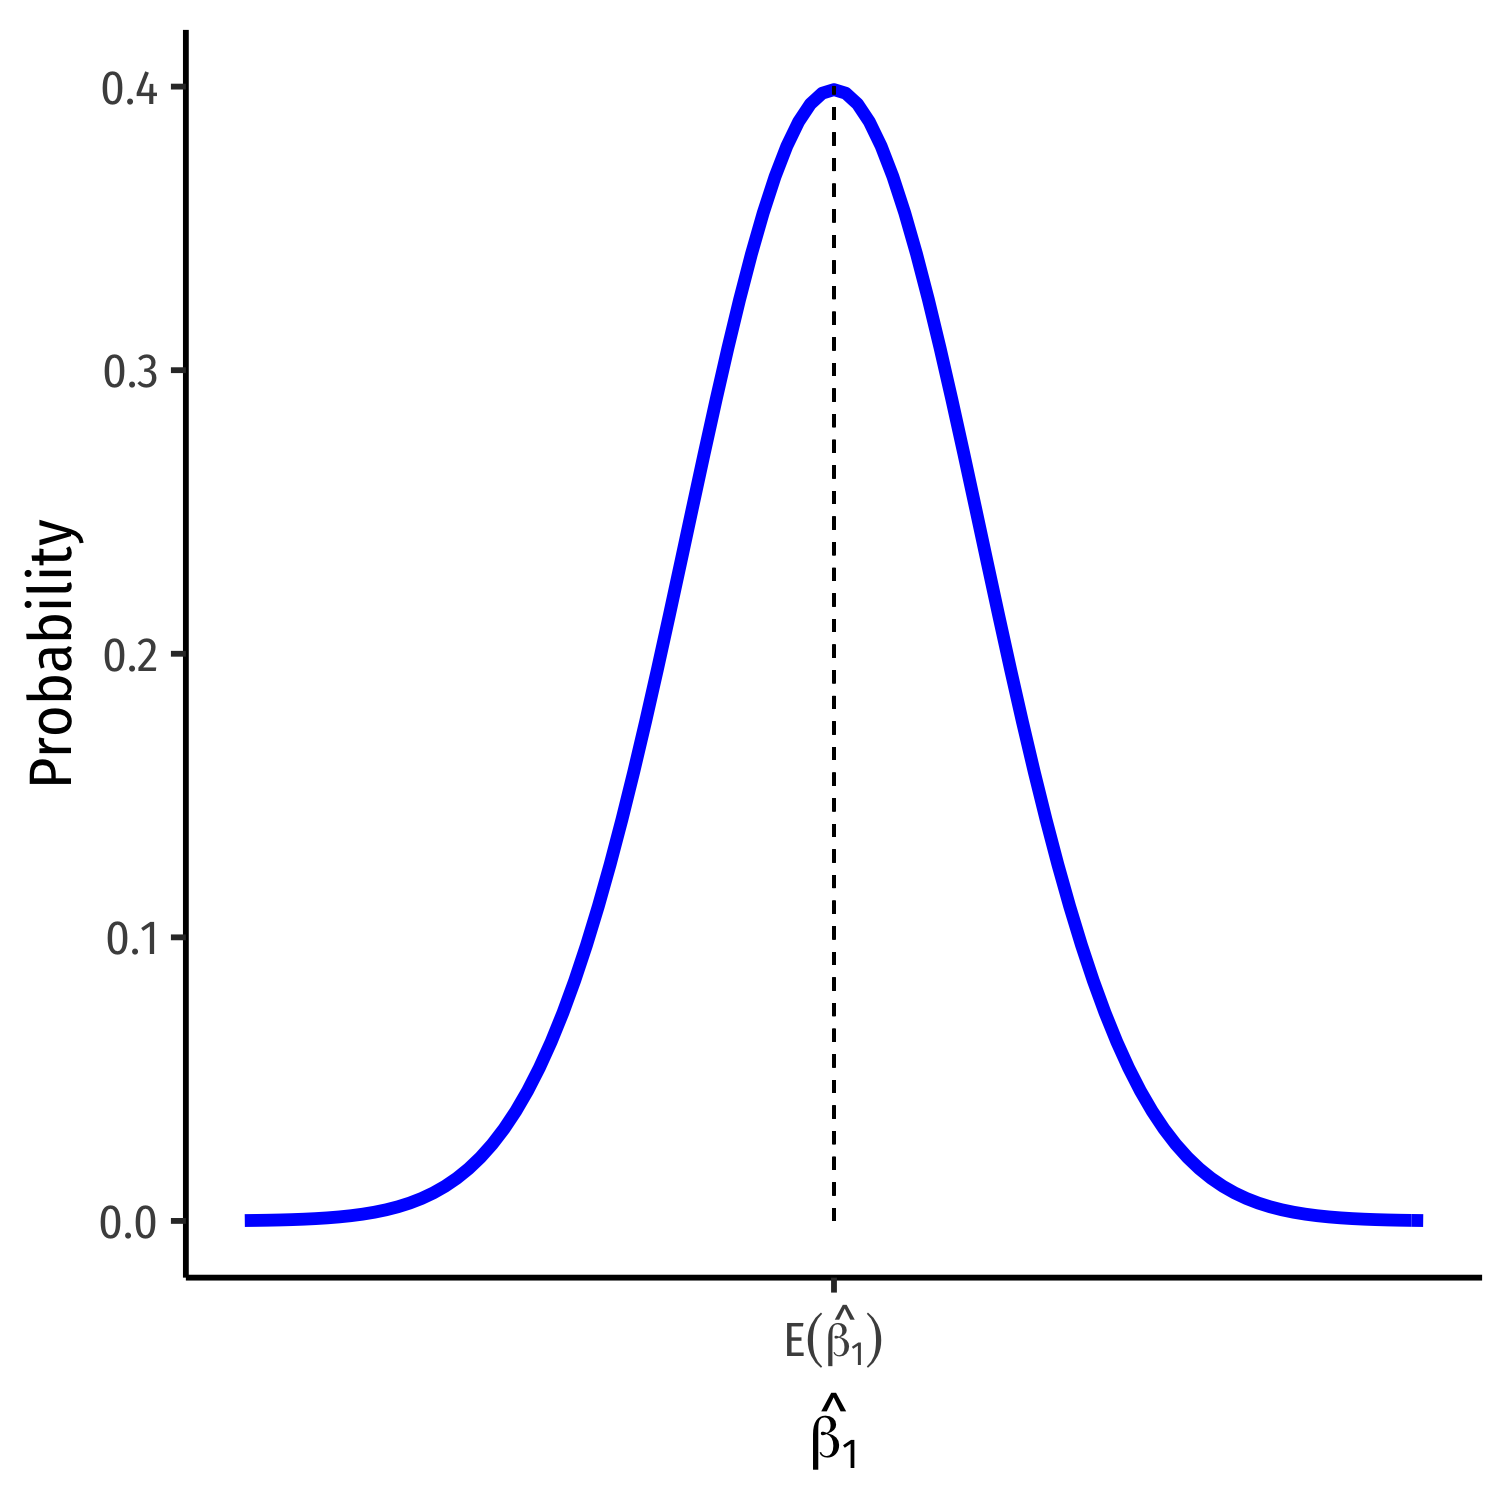
\includegraphics[width=0.8\linewidth]{04-problem-set-answers-pdf_files/figure-latex/unnamed-chunk-20-1}

\begin{center}\rule{0.5\linewidth}{0.5pt}\end{center}

\hypertarget{part-l}{%
\subsubsection{Part L}\label{part-l}}

\textbf{Estimate the causal effect in this new model by running the
appropriate regression. Compare your answers to those in part F.}

\begin{center}\rule{0.5\linewidth}{0.5pt}\end{center}

We need to control for \texttt{faminc} and \texttt{motheduc}, so we put
them into the regression to estimate:

\[bwght_i=\beta_0+\beta_1 \, cigs_i+\beta_2 \,faminc_i+ \beta_3 \, motheduc_i\]

\begin{Shaded}
\begin{Highlighting}[]
\FunctionTok{lm}\NormalTok{(bwght }\SpecialCharTok{\textasciitilde{}}\NormalTok{ cigs }\SpecialCharTok{+}\NormalTok{ faminc }\SpecialCharTok{+}\NormalTok{ motheduc, }\AttributeTok{data =}\NormalTok{ bwght) }\SpecialCharTok{\%\textgreater{}\%} \FunctionTok{summary}\NormalTok{()}
\end{Highlighting}
\end{Shaded}

\begin{verbatim}
## 
## Call:
## lm(formula = bwght ~ cigs + faminc + motheduc, data = bwght)
## 
## Residuals:
##     Min      1Q  Median      3Q     Max 
## -96.064 -11.585   0.668  13.154 150.078 
## 
## Coefficients:
##              Estimate Std. Error t value Pr(>|t|)    
## (Intercept) 116.83485    3.13778  37.235  < 2e-16 ***
## cigs         -0.46335    0.09275  -4.996 6.61e-07 ***
## faminc        0.09147    0.03246   2.818   0.0049 ** 
## motheduc      0.01426    0.25799   0.055   0.9559    
## ---
## Signif. codes:  0 '***' 0.001 '**' 0.01 '*' 0.05 '.' 0.1 ' ' 1
## 
## Residual standard error: 20.08 on 1383 degrees of freedom
##   (1 observation deleted due to missingness)
## Multiple R-squared:  0.02977,    Adjusted R-squared:  0.02767 
## F-statistic: 14.15 on 3 and 1383 DF,  p-value: 4.385e-09
\end{verbatim}

Controlling for income and education, each cigarette smoked while
pregant will cause the birthweight to decrease by 0.46 ounces. It turns
out there was no noticeable difference when we included education!

\begin{center}\rule{0.5\linewidth}{0.5pt}\end{center}

\hypertarget{part-m}{%
\subsubsection{Part M}\label{part-m}}

\textbf{Try out drawing this model using the \texttt{ggdag} package in
R. See my DAG in question 3 for an example.}

\begin{center}\rule{0.5\linewidth}{0.5pt}\end{center}

\begin{Shaded}
\begin{Highlighting}[]
\FunctionTok{library}\NormalTok{(ggdag)}
\FunctionTok{dagify}\NormalTok{(bwght }\SpecialCharTok{\textasciitilde{}}\NormalTok{ cigs }\SpecialCharTok{+}\NormalTok{ inc }\SpecialCharTok{+}\NormalTok{ educ,}
\NormalTok{       cigs }\SpecialCharTok{\textasciitilde{}}\NormalTok{ price }\SpecialCharTok{+}\NormalTok{ educ }\SpecialCharTok{+}\NormalTok{ inc,}
\NormalTok{       inc }\SpecialCharTok{\textasciitilde{}}\NormalTok{ educ }\SpecialCharTok{+}\NormalTok{ u1,}
\NormalTok{       price }\SpecialCharTok{\textasciitilde{}}\NormalTok{ u1,}
       \AttributeTok{exposure =} \StringTok{"cigs"}\NormalTok{,}
       \AttributeTok{outcome =} \StringTok{"bwght"}\NormalTok{) }\SpecialCharTok{\%\textgreater{}\%} 
  \FunctionTok{ggdag\_status}\NormalTok{()}\SpecialCharTok{+}
  \FunctionTok{theme\_dag\_blank}\NormalTok{()}\SpecialCharTok{+}
  \FunctionTok{theme}\NormalTok{(}\AttributeTok{legend.position =} \StringTok{"none"}\NormalTok{)}
\end{Highlighting}
\end{Shaded}

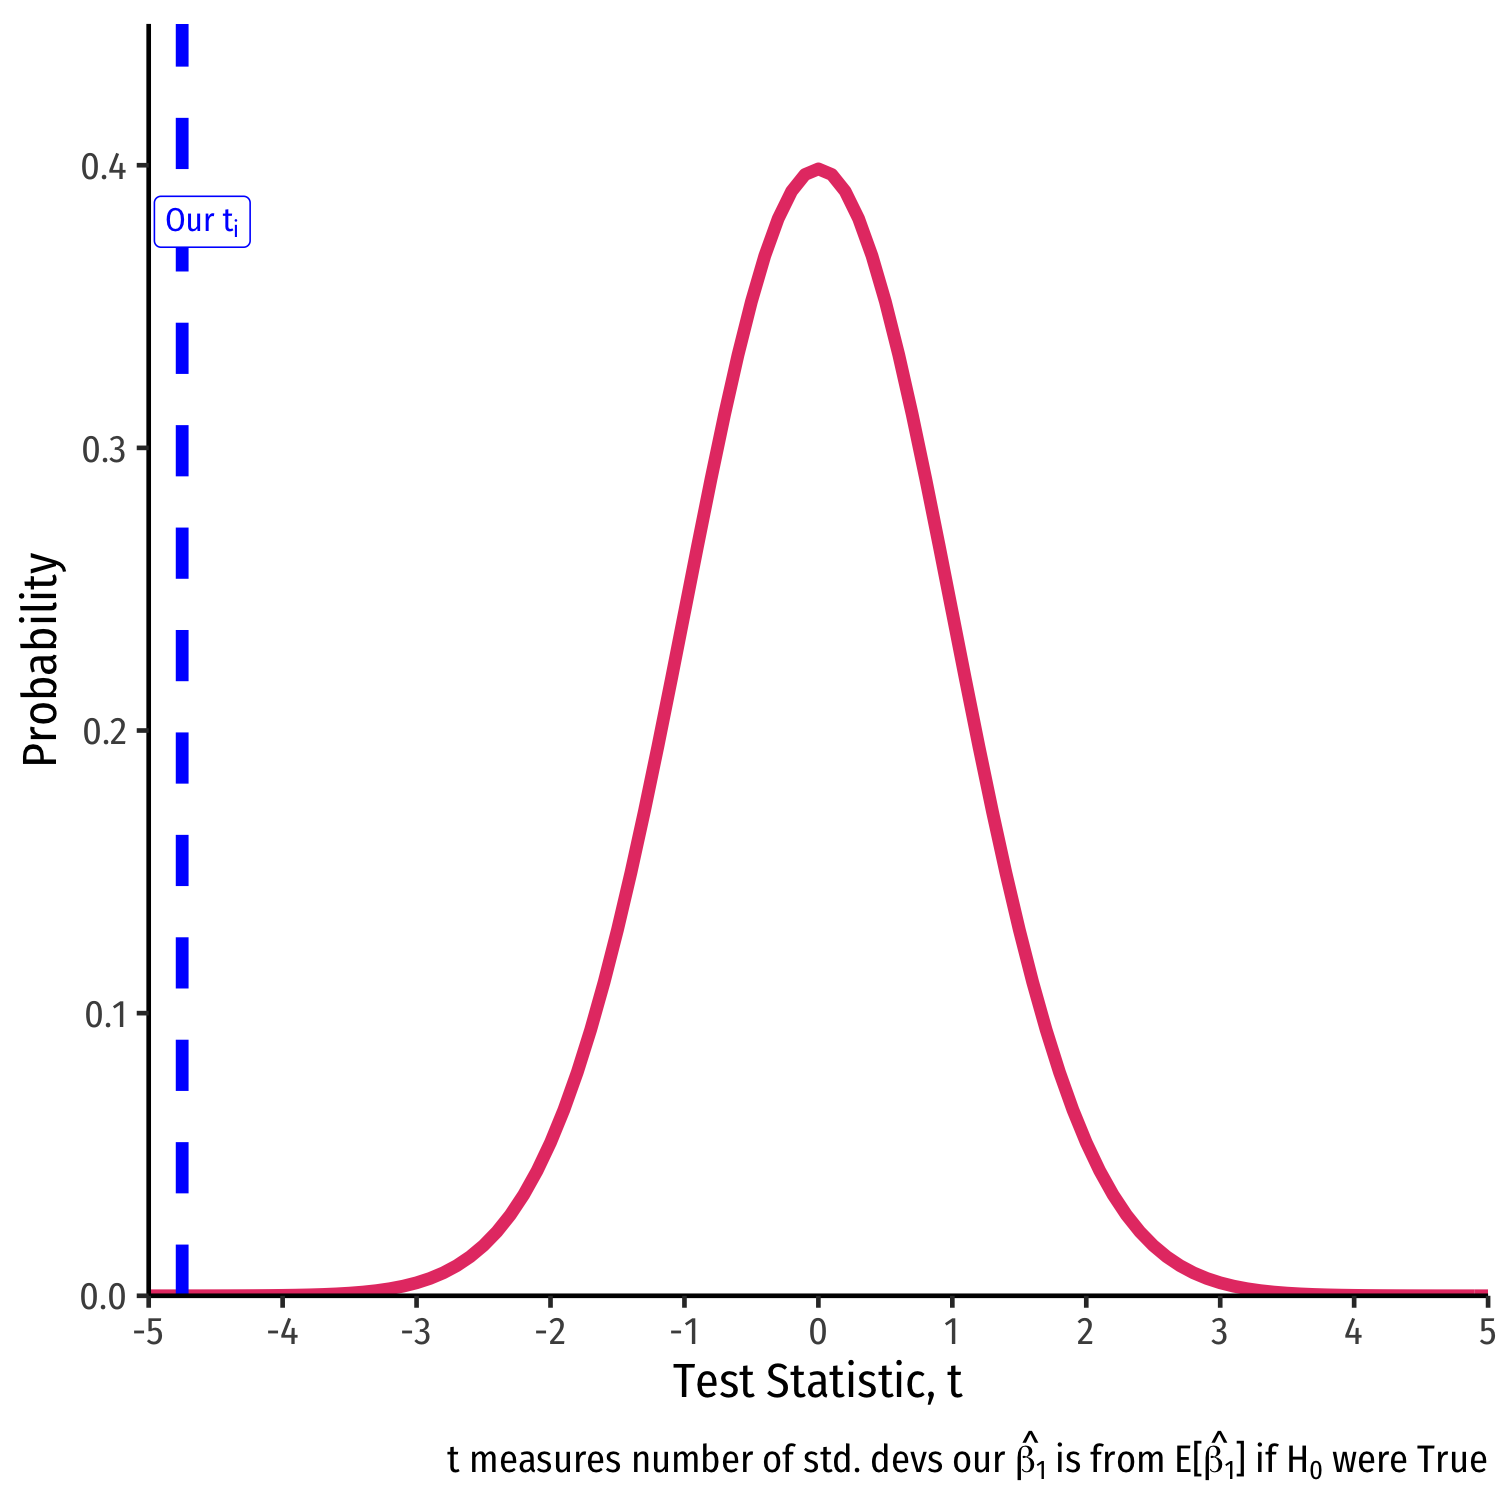
\includegraphics[width=0.8\linewidth]{04-problem-set-answers-pdf_files/figure-latex/unnamed-chunk-22-1}

\begin{center}\rule{0.5\linewidth}{0.5pt}\end{center}

\hypertarget{question-10}{%
\subsection{Question 10}\label{question-10}}

\begin{itemize}
\tightlist
\item
  \href{http://metricsf21.classes.ryansafner.com/data/heightwages.csv}{
  \texttt{heightwages.csv}}
\end{itemize}

Download the \texttt{heightwages.csv} dataset. This data is a part of a
larger dataset from the National Longitudinal Survey of Youth (NLSY)
1979 cohort: a nationally representative sample of 12,686 men and women
aged 14-22 years old when they were first surveyed in 1979. They were
subsequently interviewed every year through 1994 and then every other
year afterwards. There are many included variables, but for now we will
just focus on:

\begin{longtable}[]{@{}ll@{}}
\toprule
Variable & Description \\
\midrule
\endhead
\texttt{wage96} & Adult hourly wages (\$/hr) reported in 1996 \\
\texttt{height85} & Adult height (inches) reported in 1985 \\
\texttt{height81} & Adolescent height (inches) reported in 1981 \\
\bottomrule
\end{longtable}

\begin{quote}
We want to figure out what is the effect of height on wages (e.g.~do
taller people earn more on average than shorter people?)
\end{quote}

\hypertarget{part-a-3}{%
\subsubsection{Part A}\label{part-a-3}}

\textbf{Create a quick scatterplot between \texttt{height85} (as \(X)\)
amd \texttt{wage96} (as \(Y)\).}

\begin{center}\rule{0.5\linewidth}{0.5pt}\end{center}

\begin{Shaded}
\begin{Highlighting}[]
\CommentTok{\# load data}
\NormalTok{heights }\OtherTok{\textless{}{-}} \FunctionTok{read\_csv}\NormalTok{(}\StringTok{"https://metricsf21.classes.ryansafner.com/Data/heightwages.csv"}\NormalTok{)}
\end{Highlighting}
\end{Shaded}

\begin{verbatim}
## New names:
## * `` -> ...1
\end{verbatim}

\begin{verbatim}
## Rows: 12686 Columns: 22
\end{verbatim}

\begin{verbatim}
## -- Column specification --------------------------------------------------------
## Delimiter: ","
## dbl (22): ...1, male, white, black, hispanic, mompro2, poppro2, siblings, no...
\end{verbatim}

\begin{verbatim}
## 
## i Use `spec()` to retrieve the full column specification for this data.
## i Specify the column types or set `show_col_types = FALSE` to quiet this message.
\end{verbatim}

\begin{Shaded}
\begin{Highlighting}[]
\CommentTok{\# make scatterplot}
\FunctionTok{ggplot}\NormalTok{(}\AttributeTok{data =}\NormalTok{ heights)}\SpecialCharTok{+}
  \FunctionTok{aes}\NormalTok{(}\AttributeTok{x =}\NormalTok{ height85, }\AttributeTok{y =}\NormalTok{ wage96)}\SpecialCharTok{+}
  \FunctionTok{geom\_jitter}\NormalTok{(}\AttributeTok{color =} \StringTok{"blue"}\NormalTok{)}\SpecialCharTok{+}
  \FunctionTok{geom\_smooth}\NormalTok{(}\AttributeTok{method =} \StringTok{"lm"}\NormalTok{, }\AttributeTok{color =} \StringTok{"red"}\NormalTok{)}\SpecialCharTok{+}
  \FunctionTok{labs}\NormalTok{(}\AttributeTok{x =} \StringTok{"Adult Height in 1985 (inches)"}\NormalTok{,}
       \AttributeTok{y =} \StringTok{"Hourly Wage in 1996 ($)"}\NormalTok{)}\SpecialCharTok{+}
  \FunctionTok{theme\_classic}\NormalTok{(}\AttributeTok{base\_family =} \StringTok{"Fira Sans Condensed"}\NormalTok{,}
           \AttributeTok{base\_size =} \DecValTok{20}\NormalTok{)}
\end{Highlighting}
\end{Shaded}

\begin{verbatim}
## `geom_smooth()` using formula 'y ~ x'
\end{verbatim}

\begin{verbatim}
## Warning: Removed 5973 rows containing non-finite values (stat_smooth).
\end{verbatim}

\begin{verbatim}
## Warning: Removed 5973 rows containing missing values (geom_point).
\end{verbatim}

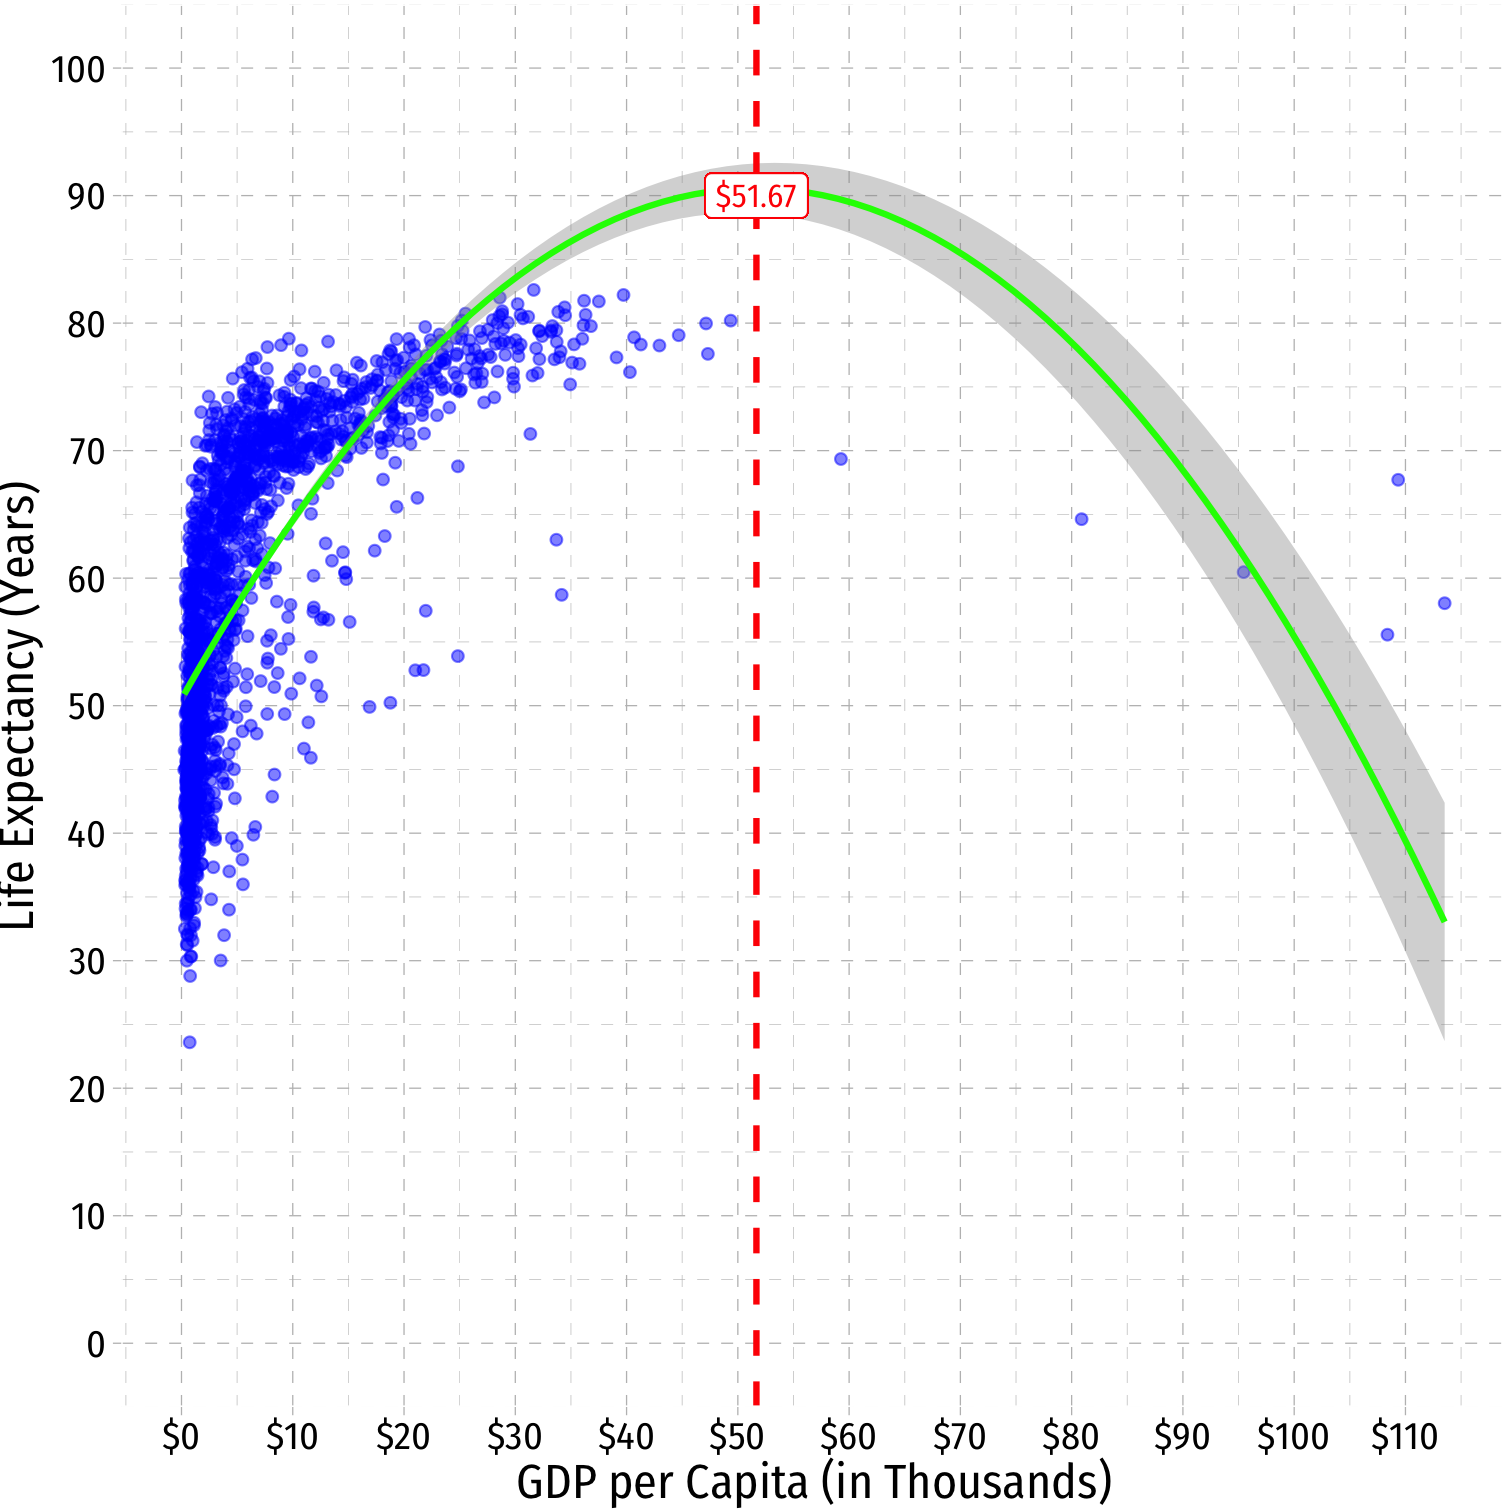
\includegraphics[width=0.8\linewidth]{04-problem-set-answers-pdf_files/figure-latex/unnamed-chunk-24-1}

\begin{center}\rule{0.5\linewidth}{0.5pt}\end{center}

\hypertarget{part-b-4}{%
\subsubsection{Part B}\label{part-b-4}}

\textbf{Regress wages on adult height. Write the equation of the
estimated OLS regression. Interpret the coefficient on
\texttt{height85}.}

\begin{center}\rule{0.5\linewidth}{0.5pt}\end{center}

\begin{Shaded}
\begin{Highlighting}[]
\NormalTok{reg1 }\OtherTok{\textless{}{-}} \FunctionTok{lm}\NormalTok{(wage96 }\SpecialCharTok{\textasciitilde{}}\NormalTok{ height85, }\AttributeTok{data =}\NormalTok{ heights)}
\FunctionTok{summary}\NormalTok{(reg1)}
\end{Highlighting}
\end{Shaded}

\begin{verbatim}
## 
## Call:
## lm(formula = wage96 ~ height85, data = heights)
## 
## Residuals:
##     Min      1Q  Median      3Q     Max 
##  -17.26   -7.21   -3.38    1.95 1520.48 
## 
## Coefficients:
##             Estimate Std. Error t value Pr(>|t|)    
## (Intercept) -6.97678    5.55895  -1.255 0.209503    
## height85     0.31475    0.08239   3.820 0.000135 ***
## ---
## Signif. codes:  0 '***' 0.001 '**' 0.01 '*' 0.05 '.' 0.1 ' ' 1
## 
## Residual standard error: 27.68 on 6711 degrees of freedom
##   (5973 observations deleted due to missingness)
## Multiple R-squared:  0.00217,    Adjusted R-squared:  0.002021 
## F-statistic: 14.59 on 1 and 6711 DF,  p-value: 0.0001346
\end{verbatim}

\(\widehat{\text{Wages}_i} = -6.98+0.31\text{Height}_i\)\$

For every additional inch in height as an adult, we can expect someone's
wages to be \$0.31 higher, on average.

\begin{center}\rule{0.5\linewidth}{0.5pt}\end{center}

\hypertarget{part-c-3}{%
\subsubsection{Part C}\label{part-c-3}}

\textbf{How much would someone who is 5'10" (70 in) be predicted to earn
per hour, according to the model?}

\begin{center}\rule{0.5\linewidth}{0.5pt}\end{center}

For a 5'10'\,' person (70 inches), they would earn:

\[\begin{align*}
    \widehat{Wages}&=-6.98+0.31Height\\
    &=-6.98+0.31(70)\\
    &=-6.98+21.70\\
    &=\$14.72\\ 
\end{align*}\]

\begin{Shaded}
\begin{Highlighting}[]
\CommentTok{\# If you want to calculate it with R}
\FunctionTok{library}\NormalTok{(broom)}

\NormalTok{reg1\_tidy }\OtherTok{\textless{}{-}} \FunctionTok{tidy}\NormalTok{(reg1)}

\NormalTok{beta\_0 }\OtherTok{\textless{}{-}}\NormalTok{ reg1\_tidy }\SpecialCharTok{\%\textgreater{}\%}
  \FunctionTok{filter}\NormalTok{(term }\SpecialCharTok{==} \StringTok{"(Intercept)"}\NormalTok{) }\SpecialCharTok{\%\textgreater{}\%}
  \FunctionTok{pull}\NormalTok{(estimate)}

\NormalTok{beta\_1 }\OtherTok{\textless{}{-}}\NormalTok{ reg1\_tidy }\SpecialCharTok{\%\textgreater{}\%}
  \FunctionTok{filter}\NormalTok{(term }\SpecialCharTok{==} \StringTok{"height85"}\NormalTok{) }\SpecialCharTok{\%\textgreater{}\%}
  \FunctionTok{pull}\NormalTok{(estimate)}

\NormalTok{beta\_0 }\SpecialCharTok{+}\NormalTok{ beta\_1}\SpecialCharTok{*}\DecValTok{70} \CommentTok{\# some rounding error in my calculation above}
\end{Highlighting}
\end{Shaded}

\begin{verbatim}
## [1] 15.05581
\end{verbatim}

\begin{center}\rule{0.5\linewidth}{0.5pt}\end{center}

\hypertarget{part-d-2}{%
\subsubsection{Part D}\label{part-d-2}}

\textbf{Would adolescent height cause an omitted variable bias if it
were left out? Explain using both your intuition, and some statistical
evidence with \texttt{R}.}

\begin{center}\rule{0.5\linewidth}{0.5pt}\end{center}

\begin{Shaded}
\begin{Highlighting}[]
\NormalTok{heights }\SpecialCharTok{\%\textgreater{}\%}
  \FunctionTok{select}\NormalTok{(wage96, height81, height85) }\SpecialCharTok{\%\textgreater{}\%}
  \FunctionTok{cor}\NormalTok{(}\AttributeTok{use =} \StringTok{"pairwise.complete.obs"}\NormalTok{)}
\end{Highlighting}
\end{Shaded}

\begin{verbatim}
##              wage96   height81   height85
## wage96   1.00000000 0.05387358 0.04658124
## height81 0.05387358 1.00000000 0.93429066
## height85 0.04658124 0.93429066 1.00000000
\end{verbatim}

We see that Adolescent height \texttt{height81} is weakly correlated
with \texttt{wage96} (to be fair, so is adult height), but it is
strongly correlated with adult height \texttt{height85}.

\begin{center}\rule{0.5\linewidth}{0.5pt}\end{center}

\hypertarget{part-e-1}{%
\subsubsection{Part E}\label{part-e-1}}

\textbf{Now add adolescent height to the regression, and write the new
regression equation below, as before. Interpret the coefficient on
\texttt{height85}.}

\begin{center}\rule{0.5\linewidth}{0.5pt}\end{center}

\begin{Shaded}
\begin{Highlighting}[]
\NormalTok{reg2 }\OtherTok{\textless{}{-}} \FunctionTok{lm}\NormalTok{(wage96 }\SpecialCharTok{\textasciitilde{}}\NormalTok{ height85 }\SpecialCharTok{+}\NormalTok{ height81, }\AttributeTok{data =}\NormalTok{ heights)}
\FunctionTok{summary}\NormalTok{(reg2)}
\end{Highlighting}
\end{Shaded}

\begin{verbatim}
## 
## Call:
## lm(formula = wage96 ~ height85 + height81, data = heights)
## 
## Residuals:
##     Min      1Q  Median      3Q     Max 
##  -17.86   -7.23   -3.40    1.99 1520.49 
## 
## Coefficients:
##             Estimate Std. Error t value Pr(>|t|)  
## (Intercept)  -9.2483     5.7749  -1.601   0.1093  
## height85     -0.1068     0.2425  -0.440   0.6598  
## height81      0.4575     0.2459   1.860   0.0629 .
## ---
## Signif. codes:  0 '***' 0.001 '**' 0.01 '*' 0.05 '.' 0.1 ' ' 1
## 
## Residual standard error: 27.89 on 6591 degrees of freedom
##   (6092 observations deleted due to missingness)
## Multiple R-squared:  0.002685,   Adjusted R-squared:  0.002383 
## F-statistic: 8.873 on 2 and 6591 DF,  p-value: 0.0001417
\end{verbatim}

\[\widehat{\text{Wages}_i}=-9.25-0.11\text{Height85}_i+0.46\text{Height81}_i\]

For every additional inch in height as an adult, we can expect someone's
wages to be \$0.11 lower, on average, holding their adolescent height
constant.

\begin{center}\rule{0.5\linewidth}{0.5pt}\end{center}

\hypertarget{part-f-1}{%
\subsubsection{Part F}\label{part-f-1}}

\textbf{How much would someone who is 5'10" in 1985 and 4'8" in 1981 be
predicted to earn, according to the model?}

\begin{center}\rule{0.5\linewidth}{0.5pt}\end{center}

For that 5'10" person (70 inches) in 1985 and 4'10" (58") in 1981, they
would earn:

\[\begin{align*}
    \widehat{Wages}&=-9.25-0.11Height85+0.46Height81\\
    &=-9.25-0.11(70)+0.46(58)\\
    &=-9.25-7.70+25.76\\
    &=\$9.73 \\ 
\end{align*}\]

\begin{Shaded}
\begin{Highlighting}[]
\CommentTok{\# If you want to calculate it with R}
\FunctionTok{library}\NormalTok{(broom)}
\NormalTok{reg2\_tidy }\OtherTok{\textless{}{-}} \FunctionTok{tidy}\NormalTok{(reg2)}

\NormalTok{multi\_beta\_0 }\OtherTok{\textless{}{-}}\NormalTok{ reg2\_tidy }\SpecialCharTok{\%\textgreater{}\%}
  \FunctionTok{filter}\NormalTok{(term }\SpecialCharTok{==} \StringTok{"(Intercept)"}\NormalTok{) }\SpecialCharTok{\%\textgreater{}\%}
  \FunctionTok{pull}\NormalTok{(estimate)}

\NormalTok{multi\_beta\_1 }\OtherTok{\textless{}{-}}\NormalTok{ reg2\_tidy }\SpecialCharTok{\%\textgreater{}\%}
  \FunctionTok{filter}\NormalTok{(term }\SpecialCharTok{==} \StringTok{"height85"}\NormalTok{) }\SpecialCharTok{\%\textgreater{}\%}
  \FunctionTok{pull}\NormalTok{(estimate)}

\NormalTok{multi\_beta\_2 }\OtherTok{\textless{}{-}}\NormalTok{ reg2\_tidy }\SpecialCharTok{\%\textgreater{}\%}
  \FunctionTok{filter}\NormalTok{(term }\SpecialCharTok{==} \StringTok{"height81"}\NormalTok{) }\SpecialCharTok{\%\textgreater{}\%}
  \FunctionTok{pull}\NormalTok{(estimate)}

\NormalTok{multi\_beta\_0 }\SpecialCharTok{+}\NormalTok{ multi\_beta\_1}\SpecialCharTok{*}\DecValTok{70} \SpecialCharTok{+}\NormalTok{ multi\_beta\_2}\SpecialCharTok{*}\DecValTok{58} \CommentTok{\# some rounding error in my calculation above}
\end{Highlighting}
\end{Shaded}

\begin{verbatim}
## [1] 9.810844
\end{verbatim}

\begin{center}\rule{0.5\linewidth}{0.5pt}\end{center}

\hypertarget{part-g-1}{%
\subsubsection{Part G}\label{part-g-1}}

\textbf{What happened to the estimate on \texttt{height85} and its
standard error?}

\begin{center}\rule{0.5\linewidth}{0.5pt}\end{center}

The effect fell by more than a half, and turned negative. The standard
error also doubled (likely due to multicollinearity).

\begin{center}\rule{0.5\linewidth}{0.5pt}\end{center}

\hypertarget{part-h-1}{%
\subsubsection{Part H}\label{part-h-1}}

\textbf{Is there multicollinearity between \texttt{height85} and
\texttt{height81}? Explore with a scatterplot. Hint: to avoid
overplotting, use \texttt{geom\_jitter()} instead of
\texttt{geom\_point()} to get a better view of the data.}

\begin{center}\rule{0.5\linewidth}{0.5pt}\end{center}

\begin{Shaded}
\begin{Highlighting}[]
\FunctionTok{ggplot}\NormalTok{(}\AttributeTok{data =}\NormalTok{ heights)}\SpecialCharTok{+}
  \FunctionTok{aes}\NormalTok{(}\AttributeTok{x =}\NormalTok{ height81, }\AttributeTok{y =}\NormalTok{ height85)}\SpecialCharTok{+}
  \FunctionTok{geom\_jitter}\NormalTok{(}\AttributeTok{color =} \StringTok{"blue"}\NormalTok{)}\SpecialCharTok{+}
  \FunctionTok{geom\_smooth}\NormalTok{(}\AttributeTok{method =} \StringTok{"lm"}\NormalTok{, }\AttributeTok{color =} \StringTok{"red"}\NormalTok{)}\SpecialCharTok{+}
  \FunctionTok{labs}\NormalTok{(}\AttributeTok{x =} \StringTok{"Adult Height in 1985 (inches)"}\NormalTok{,}
       \AttributeTok{y =} \StringTok{"Adolescent Height in 1981 (inches)"}\NormalTok{)}\SpecialCharTok{+}
  \FunctionTok{theme\_classic}\NormalTok{(}\AttributeTok{base\_family =} \StringTok{"Fira Sans Condensed"}\NormalTok{,}
           \AttributeTok{base\_size =} \DecValTok{20}\NormalTok{)}
\end{Highlighting}
\end{Shaded}

\begin{verbatim}
## `geom_smooth()` using formula 'y ~ x'
\end{verbatim}

\begin{verbatim}
## Warning: Removed 2105 rows containing non-finite values (stat_smooth).
\end{verbatim}

\begin{verbatim}
## Warning: Removed 2105 rows containing missing values (geom_point).
\end{verbatim}

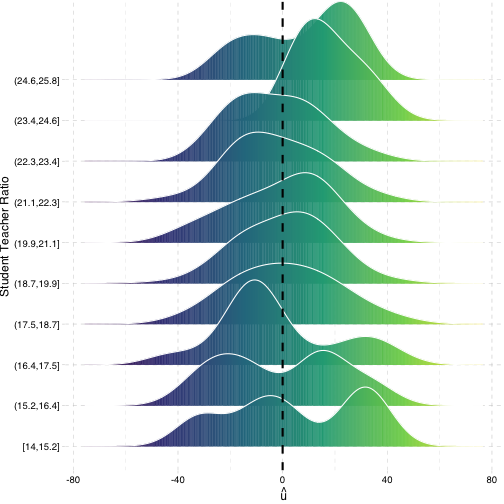
\includegraphics[width=0.8\linewidth]{04-problem-set-answers-pdf_files/figure-latex/unnamed-chunk-30-1}

\begin{center}\rule{0.5\linewidth}{0.5pt}\end{center}

\hypertarget{part-i-1}{%
\subsubsection{Part I}\label{part-i-1}}

\textbf{Quantify how much multicollinearity affects the variance of the
OLS estimates on both heights. Hint: You'll need the \texttt{vif}
command from the \texttt{car} package.}

\begin{center}\rule{0.5\linewidth}{0.5pt}\end{center}

We simply run \texttt{vif()} (from the \texttt{car} package library)
after the recent regression to calculate the Variance Inflation Factor
(VIF).

\begin{Shaded}
\begin{Highlighting}[]
\CommentTok{\#install.packages("car") \# install if you don\textquotesingle{}t have }
\FunctionTok{library}\NormalTok{(}\StringTok{"car"}\NormalTok{) }\CommentTok{\# load the car library for the vif() command}
\end{Highlighting}
\end{Shaded}

\begin{verbatim}
## Loading required package: carData
\end{verbatim}

\begin{verbatim}
## 
## Attaching package: 'car'
\end{verbatim}

\begin{verbatim}
## The following object is masked from 'package:dplyr':
## 
##     recode
\end{verbatim}

\begin{verbatim}
## The following object is masked from 'package:purrr':
## 
##     some
\end{verbatim}

\begin{Shaded}
\begin{Highlighting}[]
\FunctionTok{vif}\NormalTok{(reg2) }\CommentTok{\# run vif }
\end{Highlighting}
\end{Shaded}

\begin{verbatim}
## height85 height81 
## 8.383416 8.383416
\end{verbatim}

The variance of each OLS estimate is inflated by 8.38 times due to
multicollinearity.

\begin{center}\rule{0.5\linewidth}{0.5pt}\end{center}

\hypertarget{part-j-1}{%
\subsubsection{Part J}\label{part-j-1}}

\textbf{Reach the same number as in part I by running an auxiliary
regression.}

\textbf{Hint: There's some missing \texttt{wage96} data that may give
you a different answer, so take the data and
\texttt{filter(!is.na(wage96)} before running this regression --- this
will include only observations for \texttt{wage96} that are not
\texttt{NA}'s.}

\begin{center}\rule{0.5\linewidth}{0.5pt}\end{center}

\begin{Shaded}
\begin{Highlighting}[]
\NormalTok{aux\_reg }\OtherTok{\textless{}{-}}\NormalTok{ heights }\SpecialCharTok{\%\textgreater{}\%}
  \FunctionTok{filter}\NormalTok{(}\SpecialCharTok{!}\FunctionTok{is.na}\NormalTok{(wage96)) }\SpecialCharTok{\%\textgreater{}\%} \CommentTok{\# use only for which we have wages}
  \FunctionTok{lm}\NormalTok{(}\AttributeTok{data =}\NormalTok{ ., height85 }\SpecialCharTok{\textasciitilde{}}\NormalTok{ height81) }\CommentTok{\# run regression}

\FunctionTok{summary}\NormalTok{(aux\_reg) }\CommentTok{\# look for R{-}squared}
\end{Highlighting}
\end{Shaded}

\begin{verbatim}
## 
## Call:
## lm(formula = height85 ~ height81, data = .)
## 
## Residuals:
##      Min       1Q   Median       3Q      Max 
## -15.3510  -0.3994  -0.1574   0.6006  14.0198 
## 
## Coefficients:
##             Estimate Std. Error t value Pr(>|t|)    
## (Intercept) 3.448524   0.290169   11.88   <2e-16 ***
## height81    0.951601   0.004313  220.62   <2e-16 ***
## ---
## Signif. codes:  0 '***' 0.001 '**' 0.01 '*' 0.05 '.' 0.1 ' ' 1
## 
## Residual standard error: 1.416 on 6592 degrees of freedom
##   (336 observations deleted due to missingness)
## Multiple R-squared:  0.8807, Adjusted R-squared:  0.8807 
## F-statistic: 4.867e+04 on 1 and 6592 DF,  p-value: < 2.2e-16
\end{verbatim}

We find that adult height is positively affected by adolescent height
(\(\hat{\beta_1}=0.95\), meaning for every inch that someone is when
they are an adolescent, their adult height can be predicted to be about
the same). The \(R^2\) on the auxiliary regression is 0.88.

\[\begin{align*}
    VIF&=\frac{1}{1-R^2_1}\\
        &=\frac{1}{1-(0.8807)}\\
        &=\frac{1}{0.1193}\\
        &=8.38\\
\end{align*}\]

\begin{Shaded}
\begin{Highlighting}[]
\CommentTok{\# in R: }

\CommentTok{\# extract r.squared using broom}
\NormalTok{aux\_r\_sq }\OtherTok{\textless{}{-}} \FunctionTok{glance}\NormalTok{(aux\_reg) }\SpecialCharTok{\%\textgreater{}\%}
  \FunctionTok{pull}\NormalTok{(r.squared)}

\CommentTok{\# vif formula}
\DecValTok{1}\SpecialCharTok{/}\NormalTok{(}\DecValTok{1}\SpecialCharTok{{-}}\NormalTok{aux\_r\_sq)}
\end{Highlighting}
\end{Shaded}

\begin{verbatim}
## [1] 8.383416
\end{verbatim}

Note if you failed to tell \texttt{R} to not drop the data with NA's you
will get a different \(R^2\) and hence a different VIF than before. This
would use more observations that have data on \texttt{height81} and
\texttt{height85} but not \texttt{wage96} which would not be used in the
regression\ldots hence, a different \(n\) and \(R^2\).

\begin{center}\rule{0.5\linewidth}{0.5pt}\end{center}

\hypertarget{part-k-1}{%
\subsubsection{Part K}\label{part-k-1}}

\textbf{Make a regression table from part B and D using
\texttt{huxtable}.}

\begin{center}\rule{0.5\linewidth}{0.5pt}\end{center}

\begin{Shaded}
\begin{Highlighting}[]
\FunctionTok{library}\NormalTok{(huxtable)}
\end{Highlighting}
\end{Shaded}

\begin{verbatim}
## 
## Attaching package: 'huxtable'
\end{verbatim}

\begin{verbatim}
## The following objects are masked from 'package:ggdag':
## 
##     label, label<-
\end{verbatim}

\begin{verbatim}
## The following object is masked from 'package:dplyr':
## 
##     add_rownames
\end{verbatim}

\begin{verbatim}
## The following object is masked from 'package:ggplot2':
## 
##     theme_grey
\end{verbatim}

\begin{Shaded}
\begin{Highlighting}[]
\FunctionTok{huxreg}\NormalTok{(}\StringTok{"Wages (1996)"} \OtherTok{=}\NormalTok{ reg1,}
       \StringTok{"Wages (1996)"} \OtherTok{=}\NormalTok{ reg2,}
       \AttributeTok{coefs =} \FunctionTok{c}\NormalTok{(}\StringTok{"Constant"} \OtherTok{=} \StringTok{"(Intercept)"}\NormalTok{,}
                 \StringTok{"Adult Height (1985)"} \OtherTok{=} \StringTok{"height85"}\NormalTok{,}
                 \StringTok{"Adolescent Height (1981)"} \OtherTok{=} \StringTok{"height81"}\NormalTok{),}
       \AttributeTok{statistics =} \FunctionTok{c}\NormalTok{(}\StringTok{"N"} \OtherTok{=} \StringTok{"nobs"}\NormalTok{,}
                      \StringTok{"R{-}Squared"} \OtherTok{=} \StringTok{"r.squared"}\NormalTok{,}
                      \StringTok{"SER"} \OtherTok{=} \StringTok{"sigma"}\NormalTok{),}
       \AttributeTok{number\_format =} \DecValTok{2}\NormalTok{)}
\end{Highlighting}
\end{Shaded}

 
  \providecommand{\huxb}[2]{\arrayrulecolor[RGB]{#1}\global\arrayrulewidth=#2pt}
  \providecommand{\huxvb}[2]{\color[RGB]{#1}\vrule width #2pt}
  \providecommand{\huxtpad}[1]{\rule{0pt}{#1}}
  \providecommand{\huxbpad}[1]{\rule[-#1]{0pt}{#1}}

\begin{table}[ht]
\begin{centerbox}
\begin{threeparttable}
 \label{tab:unnamed-chunk-34}
\setlength{\tabcolsep}{0pt}
\begin{tabular}{l l l}


\hhline{>{\huxb{0, 0, 0}{0.8}}->{\huxb{0, 0, 0}{0.8}}->{\huxb{0, 0, 0}{0.8}}-}
\arrayrulecolor{black}

\multicolumn{1}{!{\huxvb{0, 0, 0}{0}}c!{\huxvb{0, 0, 0}{0}}}{\huxtpad{6pt + 1em}\centering \hspace{6pt}  \hspace{6pt}\huxbpad{6pt}} &
\multicolumn{1}{c!{\huxvb{0, 0, 0}{0}}}{\huxtpad{6pt + 1em}\centering \hspace{6pt} Wages (1996) \hspace{6pt}\huxbpad{6pt}} &
\multicolumn{1}{c!{\huxvb{0, 0, 0}{0}}}{\huxtpad{6pt + 1em}\centering \hspace{6pt} Wages (1996) \hspace{6pt}\huxbpad{6pt}} \tabularnewline[-0.5pt]


\hhline{>{\huxb{255, 255, 255}{0.4}}->{\huxb{0, 0, 0}{0.4}}->{\huxb{0, 0, 0}{0.4}}-}
\arrayrulecolor{black}

\multicolumn{1}{!{\huxvb{0, 0, 0}{0}}l!{\huxvb{0, 0, 0}{0}}}{\huxtpad{6pt + 1em}\raggedright \hspace{6pt} Constant \hspace{6pt}\huxbpad{6pt}} &
\multicolumn{1}{r!{\huxvb{0, 0, 0}{0}}}{\huxtpad{6pt + 1em}\raggedleft \hspace{6pt} -6.98\hphantom{0}\hphantom{0}\hphantom{0}\hphantom{0} \hspace{6pt}\huxbpad{6pt}} &
\multicolumn{1}{r!{\huxvb{0, 0, 0}{0}}}{\huxtpad{6pt + 1em}\raggedleft \hspace{6pt} -9.25\hphantom{0} \hspace{6pt}\huxbpad{6pt}} \tabularnewline[-0.5pt]


\hhline{}
\arrayrulecolor{black}

\multicolumn{1}{!{\huxvb{0, 0, 0}{0}}l!{\huxvb{0, 0, 0}{0}}}{\huxtpad{6pt + 1em}\raggedright \hspace{6pt}  \hspace{6pt}\huxbpad{6pt}} &
\multicolumn{1}{r!{\huxvb{0, 0, 0}{0}}}{\huxtpad{6pt + 1em}\raggedleft \hspace{6pt} (5.56)\hphantom{0}\hphantom{0}\hphantom{0} \hspace{6pt}\huxbpad{6pt}} &
\multicolumn{1}{r!{\huxvb{0, 0, 0}{0}}}{\huxtpad{6pt + 1em}\raggedleft \hspace{6pt} (5.77) \hspace{6pt}\huxbpad{6pt}} \tabularnewline[-0.5pt]


\hhline{}
\arrayrulecolor{black}

\multicolumn{1}{!{\huxvb{0, 0, 0}{0}}l!{\huxvb{0, 0, 0}{0}}}{\huxtpad{6pt + 1em}\raggedright \hspace{6pt} Adult Height (1985) \hspace{6pt}\huxbpad{6pt}} &
\multicolumn{1}{r!{\huxvb{0, 0, 0}{0}}}{\huxtpad{6pt + 1em}\raggedleft \hspace{6pt} 0.31 *** \hspace{6pt}\huxbpad{6pt}} &
\multicolumn{1}{r!{\huxvb{0, 0, 0}{0}}}{\huxtpad{6pt + 1em}\raggedleft \hspace{6pt} -0.11\hphantom{0} \hspace{6pt}\huxbpad{6pt}} \tabularnewline[-0.5pt]


\hhline{}
\arrayrulecolor{black}

\multicolumn{1}{!{\huxvb{0, 0, 0}{0}}l!{\huxvb{0, 0, 0}{0}}}{\huxtpad{6pt + 1em}\raggedright \hspace{6pt}  \hspace{6pt}\huxbpad{6pt}} &
\multicolumn{1}{r!{\huxvb{0, 0, 0}{0}}}{\huxtpad{6pt + 1em}\raggedleft \hspace{6pt} (0.08)\hphantom{0}\hphantom{0}\hphantom{0} \hspace{6pt}\huxbpad{6pt}} &
\multicolumn{1}{r!{\huxvb{0, 0, 0}{0}}}{\huxtpad{6pt + 1em}\raggedleft \hspace{6pt} (0.24) \hspace{6pt}\huxbpad{6pt}} \tabularnewline[-0.5pt]


\hhline{}
\arrayrulecolor{black}

\multicolumn{1}{!{\huxvb{0, 0, 0}{0}}l!{\huxvb{0, 0, 0}{0}}}{\huxtpad{6pt + 1em}\raggedright \hspace{6pt} Adolescent Height (1981) \hspace{6pt}\huxbpad{6pt}} &
\multicolumn{1}{r!{\huxvb{0, 0, 0}{0}}}{\huxtpad{6pt + 1em}\raggedleft \hspace{6pt} \hphantom{0}\hphantom{0}\hphantom{0}\hphantom{0}\hphantom{0}\hphantom{0}\hphantom{0} \hspace{6pt}\huxbpad{6pt}} &
\multicolumn{1}{r!{\huxvb{0, 0, 0}{0}}}{\huxtpad{6pt + 1em}\raggedleft \hspace{6pt} 0.46\hphantom{0} \hspace{6pt}\huxbpad{6pt}} \tabularnewline[-0.5pt]


\hhline{}
\arrayrulecolor{black}

\multicolumn{1}{!{\huxvb{0, 0, 0}{0}}l!{\huxvb{0, 0, 0}{0}}}{\huxtpad{6pt + 1em}\raggedright \hspace{6pt}  \hspace{6pt}\huxbpad{6pt}} &
\multicolumn{1}{r!{\huxvb{0, 0, 0}{0}}}{\huxtpad{6pt + 1em}\raggedleft \hspace{6pt} \hphantom{0}\hphantom{0}\hphantom{0}\hphantom{0}\hphantom{0}\hphantom{0}\hphantom{0} \hspace{6pt}\huxbpad{6pt}} &
\multicolumn{1}{r!{\huxvb{0, 0, 0}{0}}}{\huxtpad{6pt + 1em}\raggedleft \hspace{6pt} (0.25) \hspace{6pt}\huxbpad{6pt}} \tabularnewline[-0.5pt]


\hhline{>{\huxb{255, 255, 255}{0.4}}->{\huxb{0, 0, 0}{0.4}}->{\huxb{0, 0, 0}{0.4}}-}
\arrayrulecolor{black}

\multicolumn{1}{!{\huxvb{0, 0, 0}{0}}l!{\huxvb{0, 0, 0}{0}}}{\huxtpad{6pt + 1em}\raggedright \hspace{6pt} N \hspace{6pt}\huxbpad{6pt}} &
\multicolumn{1}{r!{\huxvb{0, 0, 0}{0}}}{\huxtpad{6pt + 1em}\raggedleft \hspace{6pt} 6713\hphantom{0}\hphantom{0}\hphantom{0}\hphantom{0}\hphantom{0}\hphantom{0}\hphantom{0} \hspace{6pt}\huxbpad{6pt}} &
\multicolumn{1}{r!{\huxvb{0, 0, 0}{0}}}{\huxtpad{6pt + 1em}\raggedleft \hspace{6pt} 6594\hphantom{0}\hphantom{0}\hphantom{0}\hphantom{0} \hspace{6pt}\huxbpad{6pt}} \tabularnewline[-0.5pt]


\hhline{}
\arrayrulecolor{black}

\multicolumn{1}{!{\huxvb{0, 0, 0}{0}}l!{\huxvb{0, 0, 0}{0}}}{\huxtpad{6pt + 1em}\raggedright \hspace{6pt} R-Squared \hspace{6pt}\huxbpad{6pt}} &
\multicolumn{1}{r!{\huxvb{0, 0, 0}{0}}}{\huxtpad{6pt + 1em}\raggedleft \hspace{6pt} 0.00\hphantom{0}\hphantom{0}\hphantom{0}\hphantom{0} \hspace{6pt}\huxbpad{6pt}} &
\multicolumn{1}{r!{\huxvb{0, 0, 0}{0}}}{\huxtpad{6pt + 1em}\raggedleft \hspace{6pt} 0.00\hphantom{0} \hspace{6pt}\huxbpad{6pt}} \tabularnewline[-0.5pt]


\hhline{}
\arrayrulecolor{black}

\multicolumn{1}{!{\huxvb{0, 0, 0}{0}}l!{\huxvb{0, 0, 0}{0}}}{\huxtpad{6pt + 1em}\raggedright \hspace{6pt} SER \hspace{6pt}\huxbpad{6pt}} &
\multicolumn{1}{r!{\huxvb{0, 0, 0}{0}}}{\huxtpad{6pt + 1em}\raggedleft \hspace{6pt} 27.68\hphantom{0}\hphantom{0}\hphantom{0}\hphantom{0} \hspace{6pt}\huxbpad{6pt}} &
\multicolumn{1}{r!{\huxvb{0, 0, 0}{0}}}{\huxtpad{6pt + 1em}\raggedleft \hspace{6pt} 27.89\hphantom{0} \hspace{6pt}\huxbpad{6pt}} \tabularnewline[-0.5pt]


\hhline{>{\huxb{0, 0, 0}{0.8}}->{\huxb{0, 0, 0}{0.8}}->{\huxb{0, 0, 0}{0.8}}-}
\arrayrulecolor{black}

\multicolumn{3}{!{\huxvb{0, 0, 0}{0}}l!{\huxvb{0, 0, 0}{0}}}{\huxtpad{6pt + 1em}\raggedright \hspace{6pt}  *** p $<$ 0.001;  ** p $<$ 0.01;  * p $<$ 0.05. \hspace{6pt}\huxbpad{6pt}} \tabularnewline[-0.5pt]


\hhline{}
\arrayrulecolor{black}
\end{tabular}
\end{threeparttable}\par\end{centerbox}

\end{table}
 

\end{document}
